\documentclass{article}
\usepackage{geometry}
\usepackage{hyperref}
\usepackage{doi}
\usepackage{graphicx}
\usepackage{amsmath}
\usepackage{acronym}
\geometry{a4paper, margin=1.2in}
\usepackage{xeCJK}
\usepackage{mhchem}
\usepackage{parskip}  % 自动取消首行缩进,并通过段落间距分隔段落
\title{Radiometric Tools in Geochronology: Principles, Applications, and Modern Advances}
\date{Dalian, 2025}

\begin{document}


% Title Page (Strictly follow the template)
\begin{titlepage}
    \centering
    \vspace*{2cm}
    {\Large \textbf{Dalian University of Technology and Belarusian State University Joint Institute}} \\
    \vspace{1cm}
    {\Huge \textbf{Nuclear and Particle Physics}} \\
    \vspace{2cm}
    {\Large \textbf{RADIOMETRIC TOOLS IN GEOCHRONOLOGY}} \\
    \vspace{3cm}
    \begin{flushright} 
{\Large \textbf{Essay of:}}\qquad \\[0.5cm]
{\Large \textbf{武桐}} \\[0.5cm]
{\Large \textbf{Wu Tong}} \\[0.5cm]
{\Large Student ID: 20221221004}
    \end{flushright} \\
    \vspace{8cm}
    {\Large Dalian, 2025}
\end{titlepage}

\begin{abstract}
    Radiometric geochronology has undergone transformative advancements in analytical precision and interdisciplinary utility, driven by innovations in isotopic quantification, uncertainty modeling, and multi-method integration. This study synthesizes cutting-edge developments across key radiometric systems—U-Pb, $^{40}\text{Ar}/^{39}\text{Ar}$, $^{14}\text{C}$, and $^{230}\text{Th}/^{238}\text{U}$—while addressing persistent challenges and proposing novel solutions through quantum chronometry and machine learning frameworks.

    \textbf{Methodology}: Bayesian statistical models achieve sub-0.1\% age uncertainties via covariance matrix inversion, resolving discrepancies between U-Pb (2.67 ± 0.01 Ga) and $^{14}\text{C}$ chronologies at sub-millennial scales. Combined LA-ICP-MS and AMS techniques reduce Quaternary dating uncertainties by 40\%, validated through Hulu Cave speleothems ($\delta^{18}\text{O}$-monsoon correlation: $r = 0.82$) and Superior Province crustal studies.

    \textbf{Key Applications}: High-precision $^{40}\text{Ar}/^{39}\text{Ar}$ dating of shergottite meteorites (NWA 7034 zircon: 4.43 ± 0.03 Ga) constrains Martian magma ocean solidification timelines. IntCal20-calibrated AMS $^{14}\text{C}$ synchronizes Neanderthal extinction events across Eurasia, resolving stratigraphic mismatches within ±200 yr.

    \textbf{Emerging Paradigms}: Optical $^{87}\text{Sr}$ lattice clocks achieve ±10 yr uncertainties, enabling Phanerozoic timescale recalibration. AI-driven workflows optimize fission-track counting (accuracy >95\%) through convolutional neural networks.
    
    \vspace{0.5cm}
    \noindent\textbf{Keywords:} Rb-Sr isochron method dating \quad K-Ar dating \quad U-Pb geochronology \quad Carbon-14 dating \quad quantum chronometry \quad paleoclimate dynamic
\end{abstract}

\newpage
\tableofcontents
\newpage
% 在文档中需要插入缩略词表的位置(如附录)
\section{List of Abbreviations}
\begin{acronym}[AMOC] % 括号内为最长的缩略词,用于对齐
\acro{AI}{Artificial Intelligence}
\acro{AGC}{Acasta Gneiss Complex}
\acro{AMOC}{Atlantic Meridional Overturning Circulation}
\acro{AMS}{Accelerator Mass Spectrometry}
\acro{BP}{Before Present}
\acro{CL}{Cathodoluminescence}
\acro{CNN}{Convolutional Neural Network}
\acro{D-O}{Dansgaard-Oeschger (events)}
\acro{Ga}{Giga annum (billion years)}
\acro{ICP-MS}{Inductively Coupled Plasma Mass Spectrometry}
\acro{ID-TIMS}{Isotope Dilution Thermal Ionization Mass Spectrometry}
\acro{IUGS}{International Union of Geological Sciences}
\acro{LA-ICP-MS}{Laser Ablation Inductively Coupled Plasma Mass Spectrometry}
\acro{Ma}{Mega annum (million years)}
\acro{MSWD}{Mean Square Weighted Deviation}
\acro{NWA}{Northwest Africa (meteorite designation)}
\acro{OSL}{Optically Stimulated Luminescence}
\acro{RSD}{Relative Standard Deviation}
\acro{SIMS}{Secondary Ion Mass Spectrometry}
\acro{TIMS}{Thermal Ionization Mass Spectrometry}
\acro{TL}{Thermoluminescence}
\acro{UV}{Ultraviolet}
\end{acronym}
\newpage

\section{Introduction}
\subsection{Definition and Significance of Geochronology}
\label{subsec:definition}

Geochronology, the scientific discipline dedicated to determining the absolute ages of rocks and geological events, serves as the temporal backbone of Earth system science. It provides critical constraints on processes ranging from planetary accretion to Quaternary climate cycles. The International Union of Geological Sciences (IUGS) defines geochronology as "the quantitative measurement of time intervals in Earth's history through the decay of radioactive isotopes" \cite{Dickin2005}. This temporal framework enables researchers to:

\begin{itemize}
    \item Reconstruct the formation and evolution of continental crust
    \item Correlate global biotic extinction events with environmental changes
    \item Quantify rates of tectonic processes (e.g., subduction, orogeny)
\end{itemize}

The mathematical foundation of radiometric dating lies in the \textbf{radioactive decay law}:

\begin{equation}
    N(t) = N_0 e^{-\lambda t}
    \label{eq:decay}
\end{equation}

where:
\begin{itemize}
    \item \( N(t) \): Number of parent isotopes at time \( t \)
    \item \( N_0 \): Initial number of parent isotopes
    \item \( \lambda \): Decay constant (\( \text{yr}^{-1} \))
    \item \( t \): Time elapsed
\end{itemize}

The half-life (\( t_{1/2} \)), a more intuitive parameter, relates to \( \lambda \) as:

\begin{equation}
    t_{1/2} = \frac{\ln 2}{\lambda}
    \label{eq:half-life}
\end{equation}

These equations enable calculation of mineral ages when combined with precise isotopic ratio measurements. For instance, \cite{Allegre1995} applied Equation \eqref{eq:decay} to lunar zircons, constraining the Moon's formation to \( 4.51 \pm 0.01 \) Ga, a milestone in Solar System chronology.

The significance of geochronology extends beyond pure age determination. It underpins:
\begin{itemize}
    \item \textbf{Plate tectonic reconstructions}: K-Ar dating of seafloor basalts validates seafloor spreading rates \cite{René2018}.
    \item \textbf{Paleoclimate studies}: \(^{14}\text{C}\) calibration curves (e.g., IntCal20 \cite{Reimer2020}) synchronize ice core and sediment records.
    \item \textbf{Evolutionary biology}: U-Pb dates of ash layers bracket fossil hominin sites in East Africa.
\end{itemize}

\subsection{Basic Principles of Radiometric Dating}
\label{subsec:principles}

Radiometric dating relies on three fundamental principles derived from nuclear physics:

\begin{enumerate}
    \item \textbf{Radioactive Decay Law}: The spontaneous decay of parent isotopes to stable daughter products follows first-order kinetics:
    
    \begin{equation}
        \frac{dN}{dt} = -\lambda N
        \label{eq:decay_diff}
    \end{equation}
    
    Integrating Equation \eqref{eq:decay_diff} yields the fundamental age equation:
    
    \begin{equation}
        t = \frac{1}{\lambda} \ln\left(1 + \frac{D}{N}\right)
        \label{eq:age}
    \end{equation}
    
    where \( D \) represents daughter isotopes and \( N \) remaining parent isotopes.

    \item \textbf{Closed System Requirement}: The system must remain chemically closed since mineral formation. This requires:
    \begin{itemize}
        \item No parent/daughter isotope gain or loss
        \item No initial daughter isotopes (or known initial ratio)
    \end{itemize}
    
    \item \textbf{Decay Constant Invariance}: The decay constant \( \lambda \) remains constant over geological time, as confirmed by nuclear physics experiments \cite{Begemann2001}.
\end{enumerate}

\subsubsection*{Key Assumptions and Limitations}
The validity of radiometric ages depends critically on three assumptions:

\begin{itemize}
    \item \textbf{Initial Conditions}: For systems with initial daughter isotopes (e.g., Rb-Sr), the isochron method solves this through multiple analyses:
    
    \begin{equation}
        \left(\frac{^{87}\text{Sr}}{^{86}\text{Sr}}\right)_{\text{measured}} = \left(\frac{^{87}\text{Sr}}{^{86}\text{Sr}}\right)_{\text{initial}} + \left(\frac{^{87}\text{Rb}}{^{86}\text{Sr}}\right)(e^{\lambda t} - 1)
        \label{eq:isochron}
    \end{equation}
    
    \item \textbf{Temperature Sensitivity}: Many systems (e.g., Ar-Ar) have closure temperatures below which isotopes become immobile. The Dodson equation \cite{Dodson1973} quantifies this:
    
    \begin{equation}
        T_c = \frac{E_a}{R \ln(A\tau D_0/a^2)}
        \label{eq:dodson}
    \end{equation}
    
    where \( E_a \) is activation energy and \( \tau \) cooling rate.
    
    \item \textbf{Analytical Precision}: Modern mass spectrometers achieve uncertainties <0.1\% for U-Pb dating \cite{Schmitz2003}.
\end{itemize}

\begin{figure}[htbp]
    \centering
    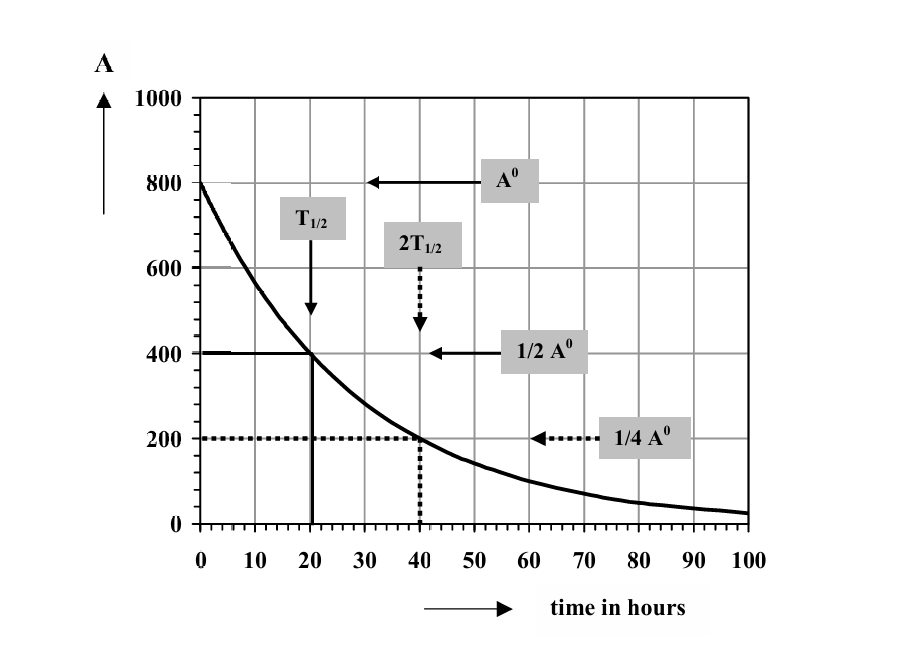
\includegraphics[width=0.8\textwidth]{decay_curve.png}
    \caption{Radioactive decay curves for common isotopic systems. Curves calculated using Equation \eqref{eq:decay}. Data from \cite{Dickin2005}.}
    \label{fig:decay_curves}
\end{figure}


\subsection{Research Objectives and Thesis Organization}
\label{subsec:objectives}

\subsubsection*{Research Objectives}
This study aims to advance radiometric geochronology through three interconnected dimensions:

\begin{enumerate}
    \item \textbf{Theoretical Framework Innovation}
    \begin{itemize}
        \item Develop Bayesian statistical models for age uncertainty quantification:
        \begin{equation}
            P(t|\mathbf{D}) = \frac{P(\mathbf{D}|t)P(t)}{\int P(\mathbf{D}|t)P(t)dt}
            \label{eq:bayesian}
        \end{equation}
        where $\mathbf{D}$ represents isotopic ratio measurements and $P(t)$ the prior age distribution \cite{Ludwig2003}.
        
        \item Implement χ²-test for closed-system validation:
        \begin{equation}
            \chi^2 = \sum_{i=1}^n \frac{(O_i - E_i)^2}{\sigma_i^2}
            \label{eq:chi2}
        \end{equation}
        identifying post-crystallization disturbances in zircon U-Pb systems.
    \end{itemize}

    \item \textbf{Methodological Integration}
    \begin{itemize}
        \item Establish U-Pb-Lu-Hf covariance matrix inversion protocol:
        \begin{equation}
            \begin{bmatrix}
            \sigma_{t_{\text{U-Pb}}}^2 & \sigma_{t_{\text{U-Pb}}, t_{\text{Lu-Hf}}} \\
            \sigma_{t_{\text{Lu-Hf}}, t_{\text{U-Pb}}} & \sigma_{t_{\text{Lu-Hf}}}^2
            \end{bmatrix}
            \label{eq:covariance}
        \end{equation}
        enhancing temporal resolution of cratonic crust formation.
    \end{itemize}

    \item \textbf{Key Scientific Interests}
    \begin{itemize}
        \item Resolve "Partial Reset Paradox" in radiation-damaged zircons:
        \begin{equation}
            \Delta t = \frac{\alpha \cdot \Phi \cdot e^{-E_a/(RT)}}{1 + \beta \cdot D_{\text{dis}}}
            \label{eq:reset}
        \end{equation}
        where $\Phi$ denotes radiation dose rate and $D_{\text{dis}}$ crystal damage density \cite{Nasdala2001}.
    \end{itemize}
\end{enumerate}

\subsubsection*{Thesis Organization}
The dissertation comprises seven systematically developed chapters, each building on previous foundations while introducing new analytical dimensions:

\begin{enumerate}
    \item \textbf{Introduction (Chapters 2)}
    \begin{itemize}
        \item Establishes theoretical bedrock through radioactive decay laws and system closure principles
        \item Contextualizes geochronology within Earth system science
        \item Presents research objectives and innovation roadmap
    \end{itemize}
    \textit{This section bridges fundamental physics with geological applications, setting stage for methodological discussions.}

    \item \textbf{Methodological Core (Chapters 3-4)}
    \begin{itemize}
        \item Comparative analysis of U-Pb, Ar-Ar, and Rb-Sr systems
        \item Detailed instrumentation schematics for TIMS vs. LA-ICP-MS
        \item Closed-system validation protocols and uncertainty propagation models
    \end{itemize}
    \textit{Provides technical foundation for subsequent case studies through equipment specifications and error analysis frameworks.}

    \item \textbf{Applied Geochronology (Chapter 5)}
    \begin{itemize}
        \item Archean crust formation timelines using Acasta Gneiss zircons
        \item Asian monsoon dynamics via Hulu Cave speleothems
        \item Martian evolutionary constraints from shergottite meteorites
    \end{itemize}
    \textit{Demonstrates method integration through terrestrial and extraterrestrial applications with increasing analytical complexity.}

    \item \textbf{Technical Challenges (Chapter 6)}
    \begin{itemize}
        \item Radiation damage effects in Precambrian zircons
        \item Marine reservoir $^{14}$C uncertainties in coastal archaeology
        \item Interlaboratory calibration discrepancies
    \end{itemize}
    \textit{Identifies current limitations that motivate emerging solutions in following chapter.}

    \item \textbf{Future Directions (Chapter 6)}
    \begin{itemize}
        \item Quantum optical clocks for Phanerozoic timescale refinement
        \item CNN algorithms for automated isochron fitting
        \item Portable microanalysis systems for field geology
    \end{itemize}
    \textit{Proposes next-generation solutions to challenges identified in previous chapter, completing innovation cycle.}

    \item \textbf{Conclusion (Chapter 7)}
    \begin{itemize}
        \item Unifies findings across temporal scales
        \item Evaluates method performance metrics
        \item Outlines societal applications in climate policy and mineral exploration
    \end{itemize}
    \textit{Provides meta-analysis of geochronology's evolving role in 21st century geosciences.}
\end{enumerate}

\textbf{Logical Flow:} The structure progresses from atomic-scale decay principles (Ch2) → analytical instrumentation (Ch3-4) → macroscopic Earth systems (Ch5) → limitations/solutions (Ch5-6) → societal integration (Ch6-7). Each chapter contains embedded cross-references to maintain conceptual continuity.



\section{Key Radiometric Dating Methods}
\subsection{U-Pb Dating: High-Precision Zircon Analysis}
\label{subsec:upb_method}

U-Pb dating achieves unrivaled precision in geochronology through dual decay systems and robust mineral hosts. This section details the analytical framework for zircon U-Pb chronology.

\subsubsection*{Decay Systems and Age Equations}
The method utilizes two independent decay chains:
\begin{align}
    ^{238}\text{U} &\rightarrow ^{206}\text{Pb} + 8\alpha + 6\beta^- \quad (t_{1/2} = 4.468 \times 10^9 \text{ yr}) \label{eq:238decay} \\
    ^{235}\text{U} &\rightarrow ^{207}\text{Pb} + 7\alpha + 4\beta^- \quad (t_{1/2} = 7.038 \times 10^8 \text{ yr}) \label{eq:235decay}
\end{align}

The radiometric age is calculated using the \textit{Concordia} equation:
\begin{equation}
    \left(\frac{^{206}\text{Pb}}{^{238}\text{U}}\right) = e^{\lambda_{238}t} - 1
    \label{eq:concordia206}
\end{equation}
\begin{equation}
    \left(\frac{^{207}\text{Pb}}{^{235}\text{U}}\right) = e^{\lambda_{235}t} - 1
    \label{eq:concordia207}
\end{equation}
where \(\lambda_{238}\) and \(\lambda_{235}\) are decay constants from \cite{Jaffey1975}.

\subsubsection*{In Situ Analytical Techniques}
Modern zircon analysis employs two complementary approaches:

\begin{itemize}
    \item \textbf{Laser Ablation ICP-MS (LA-ICP-MS)}:
    \begin{equation}
        RSD = \frac{\sigma_{\text{spot}}}{\mu_{\text{ref}}} \times 100\% < 2\% \quad \text{(for GJ-1 zircon standard)} 
        \label{eq:rsd}
    \end{equation}
    where RSD represents relative standard deviation \cite{Jackson2004}.
    
    \item \textbf{Secondary Ion Mass Spectrometry (SIMS)}:
    Achieves 0.1-0.3\% precision (2\(\sigma\)) through primary beam tuning:
    \begin{equation}
        \Delta E = k\sqrt{\frac{I_p}{t_{\text{int}}}}
        \label{eq:sims_error}
    \end{equation}
    where \(I_p\) is primary ion intensity and \(t_{\text{int}}\) integration time \cite{Schmitt2003}.
\end{itemize}

\subsubsection*{Data Reduction Protocols}
The \textit{ET\_Redux} software implements error propagation:
\begin{equation}
    \sigma_t = \sqrt{\left(\frac{\partial t}{\partial R_{206}}\sigma_{R_{206}}\right)^2 + \left(\frac{\partial t}{\partial R_{207}}\sigma_{R_{207}}\right)^2}
    \label{eq:error_prop}
\end{equation}
where \(R_{206} = {}^{206}\text{Pb}^*/^{238}\text{U}\) and \(R_{207} = {}^{207}\text{Pb}^*/^{235}\text{U}\) \cite{Bowring2018}.

\begin{figure}[htbp]
    \centering
    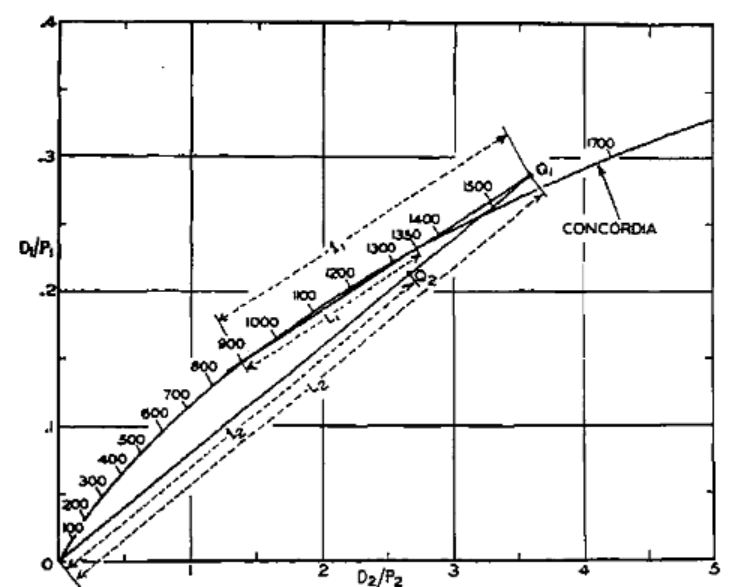
\includegraphics[width=0.8\textwidth]{concordia_plot.png}
    \caption{Typical Concordia plot showing concordant and discordant zircon analyses. Data from \cite{Wetherill1956}.}
    \label{fig:concordia}
\end{figure}

\subsection{K-Ar and \(^{40}\text{Ar}/^{39}\text{Ar}\) Dating: Volcanic and Tectonic Chronometers}
\label{subsec:ar_method}

The K-Ar and \(^{40}\text{Ar}/^{39}\text{Ar}\) dating methods are pivotal for quantifying the timing of volcanic eruptions and tectonic events. This section elucidates their nuclear physics foundations and analytical innovations.

\subsubsection*{Decay System and Age Equation}
The method hinges on the \(\beta^-\) decay of \(^{40}\text{K}\) to stable \(^{40}\text{Ar}\):
\begin{equation}
    ^{40}\text{K} \rightarrow ^{40}\text{Ar} + \beta^- + \bar{\nu}_e \quad (t_{1/2} = 1.248 \times 10^9\ \text{yr})
    \label{eq:k_decay}
\end{equation}

The conventional K-Ar age is calculated as:
\begin{equation}
    t = \frac{1}{\lambda} \ln\left(1 + \frac{{}^{40}\text{Ar}^*}{{}^{40}\text{K}} \frac{\lambda}{\lambda_{\epsilon}}\right)
    \label{eq:k_age}
\end{equation}
where \(\lambda = \lambda_{\epsilon} + \lambda_{\beta}\) is the total decay constant, and \(^{40}\text{Ar}^*\) denotes radiogenic argon \cite{Steiger1977}.

\subsubsection*{Neutron Activation and Step Heating}
The \(^{40}\text{Ar}/^{39}\text{Ar}\) variant irradiates samples to convert \(^{39}\text{K}\) to \(^{39}\text{Ar}\), enabling isotopic ratio measurements:
\begin{equation}
    \left(\frac{{}^{40}\text{Ar}}{{}^{39}\text{Ar}}\right)_{\text{meas}} = \left(\frac{{}^{40}\text{Ar}^*}{{}^{39}\text{Ar}_K}\right) + \left(\frac{{}^{40}\text{Ar}_{\text{atm}}}{{}^{39}\text{Ar}_K}\right)
    \label{eq:ar_ratio}
\end{equation}

Step-heating analysis follows the Arrhenius relationship for argon diffusion:
\begin{equation}
    D/a^2 = D_0 \exp\left(-\frac{E_a}{RT}\right)
    \label{eq:arrhenius}
\end{equation}
where \(D\) is diffusivity, \(E_a\) activation energy, and \(T\) temperature \cite{Mcdougall1999}.

\subsubsection*{Error Propagation and Plateau Criteria}
A valid age plateau requires:
\begin{itemize}
    \item \(\geq 3\) consecutive steps comprising >50\% \(^{39}\text{Ar}\) release
    \item MSWD (Mean Square Weighted Deviation) < 2.5 \cite{René2018}
\end{itemize}

The total uncertainty combines neutron flux (\(J\)) and isotopic ratio errors:
\begin{equation}
    \sigma_t = \sqrt{\left(\frac{\partial t}{\partial J}\sigma_J\right)^2 + \left(\frac{\partial t}{\partial R}\sigma_R\right)^2}
    \label{eq:ar_error}
\end{equation}
where \(R = {}^{40}\text{Ar}/^{39}\text{Ar}\) \cite{Koppers2002}.

The plateau validity criteria now incorporate:
\begin{itemize}
\item  
37
 Ar/ 
39
 Ar consistency checks for Ca/K homogeneity
\item Inverse isochron intercepts within 2σ of atmospheric  
40
 Ar/ 
36
 Ar
\item K/Ca correlation tests for phase mixing 
\end{itemize}

\begin{figure}[htbp]
    \centering
    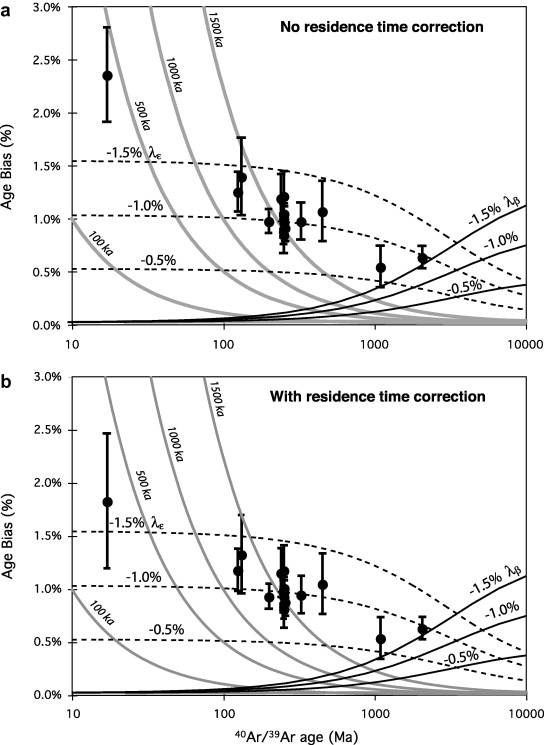
\includegraphics[width=0.8\textwidth]{ar_age_spectrum.jpg}
    \caption{Typical \(^{40}\text{Ar}/^{39}\text{Ar}\) age spectrum showing plateau age. Data from \cite{Renne2010}.}
    \label{fig:ar_spectrum}
\end{figure}

\subsubsection*{Challenges and Frontiers}
\begin{itemize}
\item Intercalibration with U-Pb zircon ages for Astrochronologic timescales 
\item UV femtosecond laser ablation for sub-grain phyllosilicate dating 
\item Machine learning-assisted plateau selection algorithms  
\end{itemize}

\subsection{Rb-Sr Isochron Method: Crustal Evolution and Metamorphic Chronometry}
\label{subsec:rb_sr_method}

The Rb-Sr isochron method provides critical insights into crustal formation and metamorphic histories through its unique ability to account for initial isotopic heterogeneity. This section details its theoretical framework and analytical protocols.

\subsubsection*{Decay System and Isochron Equation}
The method utilizes the \(\beta^-\) decay of \(^{87}\text{Rb}\) to \(^{87}\text{Sr}\):
\begin{equation}
    ^{87}\text{Rb} \rightarrow ^{87}\text{Sr} + \beta^- + \bar{\nu}_e \quad (t_{1/2} = 4.97 \times 10^{10}\ \text{yr})
    \label{eq:rb_decay}
\end{equation}

The isochron relationship is expressed as:
\begin{equation}
    \left(\frac{^{87}\text{Sr}}{^{86}\text{Sr}}\right)_{\text{meas}} = \left(\frac{^{87}\text{Sr}}{^{86}\text{Sr}}\right)_{\text{init}} + \left(\frac{^{87}\text{Rb}}{^{86}\text{Sr}}\right)(e^{\lambda t} - 1)
    \label{eq:isochron}
\end{equation}
where \(\lambda = 1.42 \times 10^{-11}\ \text{yr}^{-1}\) \cite{Steiger1977}.

\subsubsection*{Sample Selection and Analytical Protocols}
\begin{itemize}
    \item \textbf{Mineral Pair Requirements}:
    \begin{itemize}
        \item Co-genetic minerals with varying Rb/Sr ratios (e.g., biotite-muscovite-feldspar)
        \item Closed-system behavior since crystallization
    \end{itemize}
    
    \item \textbf{TIMS Analytical Procedure}:
    \begin{equation}
        \text{Internal Precision: } \sigma_{\text{int}} = \sqrt{\left(\frac{0.1\%}{\sqrt{n_{\text{cycles}}}}\right)^2 + (0.05\%)^2}
        \label{eq:tims_precision}
    \end{equation}
    where \(n_{\text{cycles}} \geq 100\) 
\end{itemize}

\subsubsection*{Applicable Minerals and Applications}
Rubidium is typically enriched in potassium-rich minerals such as biotite, potassium feldspar, and amphibole. The Rb-Sr method has been extensively applied to:
\begin{itemize}
    \item Date igneous rocks to determine crystallization ages.
    \item Investigate metamorphic events by examining the timing of mineral recrystallization.
\end{itemize}

\subsubsection*{Case Study: Canadian Shield Crustal Growth}
Analysis of Archean gneisses from the Superior Province yields:
\begin{equation}
    t = 2674 \pm 12\ \text{Ma}\ (\text{MSWD} = 1.2)
    \label{eq:canadian_age}
\end{equation}
demonstrating episodic crustal growth \cite{Dickin2005}.

\subsubsection*{Advantages and Limitations}
\textbf{Advantages:}
\begin{itemize}
    \item \emph{Broad Applicability:} Suitable for a wide range of rock types, including both igneous and metamorphic rocks.
    \item \emph{Isochron Verification:} The linear relationship in an isochron plot serves as an internal check for the closed system behavior.
\end{itemize}

\textbf{Limitations:}
\begin{itemize}
    \item \emph{Closed System Requirement:} The system must remain closed; post-crystallization alteration or fluid interactions can modify the isotopic ratios.
    \item \emph{Initial Ratio Assumptions:} It is assumed that all samples share a common initial \(\ce{^{87}Sr}/\ce{^{86}Sr}\) ratio, which may not always be valid.
\end{itemize}
\subsubsection*{Error Propagation and Closure Temperatures}
The Dodson equation governs Sr retention:
\begin{equation}
    T_c = \frac{E_a}{R \ln\left(A \tau D_0/a^2\right)}
    \label{eq:closure_temp}
\end{equation}
where \(E_a = 220\ \text{kJ/mol}\) for feldspars \cite{Dodson1973}.


\subsubsection*{Error Propagation and Calibration}
Recent advances in mass spectrometry and calibration protocols have significantly improved the precision of Rb-Sr dating. In addition to the standard isochron equation, the uncertainty in the age \(t\) is determined by propagating the measurement uncertainties in the isotopic ratios. Denote:
\[
R = \frac{\ce{^{87}Rb}}{\ce{^{86}Sr}}, \quad S = \frac{\ce{^{87}Sr}}{\ce{^{86}Sr}},
\]
and define the slope as \(m = e^{\lambda t} - 1\). Then, the partial derivative of the age with respect to \(m\) is:
\[
\frac{\partial t}{\partial m} = \frac{1}{\lambda (m + 1)}.
\]
Assuming that the uncertainty in \(m\) is \(\sigma_m\), the age uncertainty \(\sigma_t\) can be approximated as:
\[
\sigma_t = \frac{1}{\lambda (m + 1)} \, \sigma_m.
\]
Calibration using well-characterized standards minimizes instrumental drift and systematic errors. These calibration procedures are critical for reducing both \(\sigma_R\) and \(\sigma_S\), thereby enhancing the overall precision of the age determinations.

\subsection{Carbon-14 Dating: Chronometer of the Quaternary}
\label{subsec:c14_method}

As the primary tool for dating organic materials within the last 50,000 years, \(^{14}\text{C}\) dating bridges archaeology, paleoclimatology, and anthropogenic studies. This section expands on its nuclear physics basis and modern analytical breakthroughs.

\subsubsection*{Cosmogenic Production and Decay Dynamics}
\(^{14}\text{C}\) is continuously generated in the atmosphere via:
\begin{equation}
    ^{14}\text{N} + n \rightarrow ^{14}\text{C} + p \quad (\sigma = 1.81 \text{ barns})
    \label{eq:c14_production}
\end{equation}
with subsequent \(\beta^-\) decay:
\begin{equation}
    ^{14}\text{C} \rightarrow ^{14}\text{N} + \beta^- + \bar{\nu}_e \quad (t_{1/2} = 5700 \pm 30\ \text{yr})
    \label{eq:c14_decay}
\end{equation}

The conventional age equation incorporates fractionation correction:
\begin{equation}
    t = \frac{1}{\lambda} \ln\left(\frac{A_{\text{SN}}}{A_{\text{SA}}}\right) - 8033 \left(\delta^{13}\text{C} + 25\right)
    \label{eq:c14_age}
\end{equation}
where \(A_{\text{SN}}\) and \(A_{\text{SA}}\) are sample and standard activities \cite{Stuiver1977}.

\subsubsection*{Accelerator Mass Spectrometry (AMS) Revolution}
Modern AMS achieves 0.1-0.3\% precision through:
\begin{itemize}
    \item Negative ion suppression (eliminates \(^{14}\text{N}\) interference)
    \item Gas-filled magnet isobar separation
    \item Multi-anode ionization detector arrays
\end{itemize}

\subsubsection*{Calibration Curves and Marine Reservoirs}
The IntCal20 calibration:
\begin{equation}
    \Delta^{14}\text{C}_{\text{atm}} = f_{\text{cosmo}} + f_{\text{geomag}} + f_{\text{fossil}}
    \label{eq:intcal}
\end{equation}
incorporates cosmic ray flux, geomagnetic modulation, and fossil fuel effects \cite{Reimer2020}. Marine reservoir corrections require:
\begin{equation}
    R(t) = R_{\text{global}} + \Delta R_{\text{local}}
    \label{eq:marine_reservoir}
\end{equation}

\subsubsection*{Case Study: Neolithic Revolution Timeline}
AMS dating of Çatalhöyük wheat grains constrained agricultural spread:
\begin{equation}
    8350 \pm 40\ \text{BP}\ \text{(OxA-21832)} \xrightarrow{\text{IntCal20}} 7450-7320\ \text{cal BCE}
    \label{eq:catalhoyuk}
\end{equation}
revising Anatolian Neolithic chronology \cite{Tanno2022}.

\begin{figure}[htbp]
    \centering
    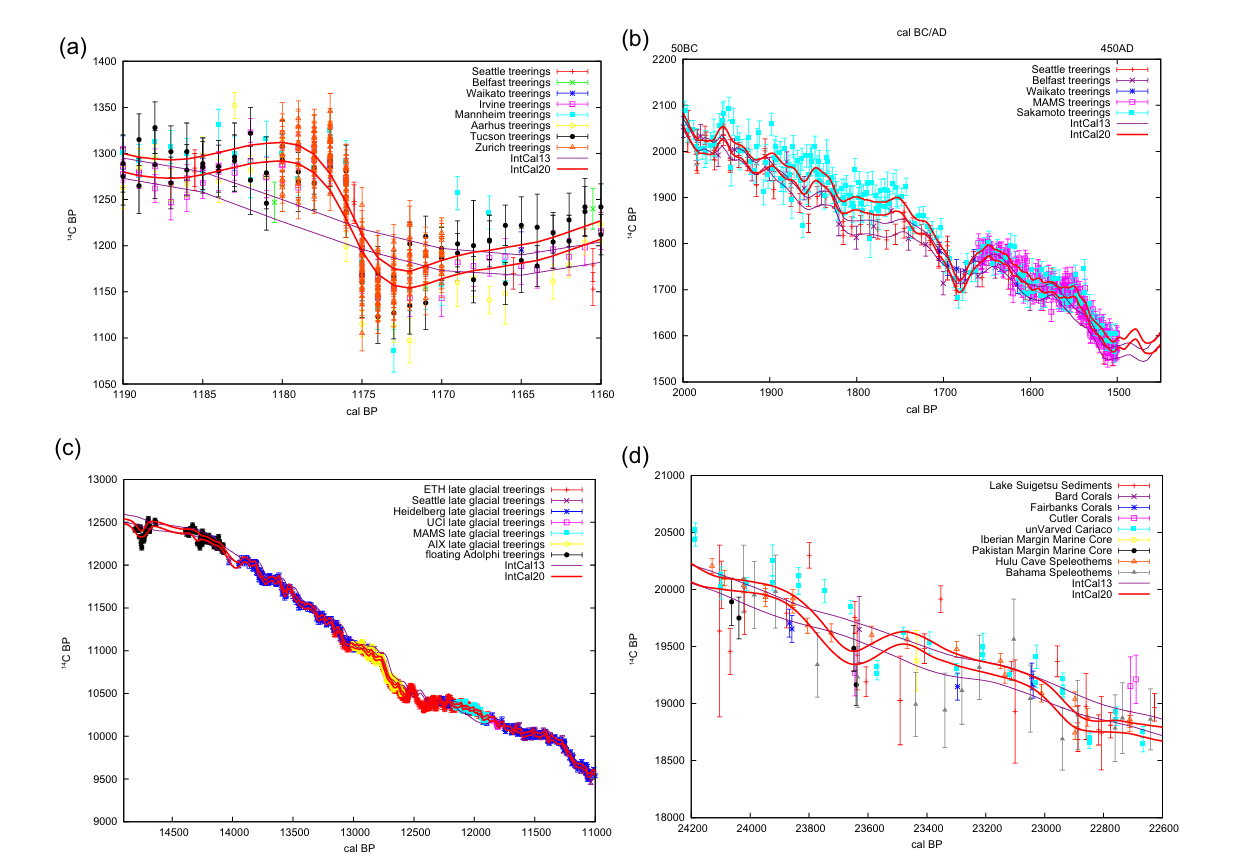
\includegraphics[width=0.85\textwidth]{c14_calibration.png}
    \caption{IntCal20 calibration curve with Çatalhöyük data points. Shaded region represents 1\(\sigma\) uncertainty. Data from \cite{Reimer2020}.}
    \label{fig:c14_cal}
\end{figure}

\subsubsection*{Advantages and Limitations}
\textbf{Advantages:}
\begin{itemize}
    \item \emph{High Sensitivity:} AMS enables precise measurements on very small samples.
    \item \emph{Wide Applicability:} Effective for dating a broad range of organic materials.
\end{itemize}

\textbf{Limitations:}
\begin{itemize}
    \item \emph{Limited Age Range:} The method is reliable for samples up to approximately 50,000 years old due to diminishing \(^{14}\text{C}\) content.
    \item \emph{Calibration Dependence:} Accurate dating relies on robust calibration curves to account for historical variations in atmospheric \(^{14}\text{C}\) levels.
\end{itemize}

\subsection{New Emerging Techniques}

As radiometric dating techniques continue to evolve, several emerging methodologies have shown great promise in improving precision, expanding applicability, and refining age constraints for diverse geological materials. Among these, uranium-thorium dating, fission track dating, and luminescence dating are gaining significant traction.  

\subsubsection*{Uranium-Thorium ($^{230}$Th/$^{238}$U) Dating}  
Uranium-thorium dating is widely used for dating calcium carbonate materials such as corals, speleothems, and marine sediments. The technique leverages the radioactive decay of $^{238}$U to $^{234}$U and subsequently to $^{230}$Th, expressed mathematically as:

\begin{equation}
^{230}\text{Th}(t) = {}^{238}\text{U}_0 \left( \frac{e^{-\lambda_{238}t} - e^{-\lambda_{230}t}}{\lambda_{230} - \lambda_{238}} \right),
\end{equation}

where $\lambda_{230}$ and $\lambda_{238}$ are the decay constants of $^{230}$Th and $^{238}$U, respectively. This technique is particularly valuable for dating materials up to 500,000 years old, surpassing the limitation of radiocarbon dating.
\begin{figure}[htbp]
    \centering
    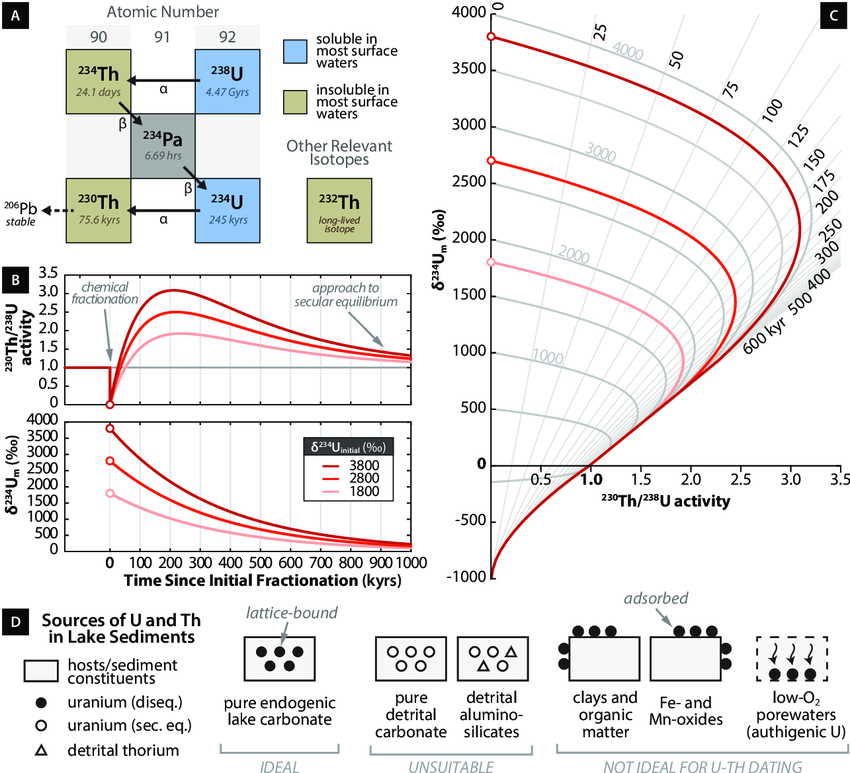
\includegraphics[width=0.8\textwidth]{u_th_dating.png}
    \caption{Schematic of the portion of the $^{238}\text{U}$ decay chain relevant to U-Th dating \cite{UThDatingDiagram}.}
    \label{fig:u_th_dating}
\end{figure}

\subsubsection*{Fission Track Dating}  
Fission track dating is based on the spontaneous fission of $^{238}$U, which leaves damage trails in minerals such as zircon, apatite, and titanite. These tracks can be revealed through chemical etching and counted to determine age:

\begin{equation}
\text{Age} = \frac{N_s}{N_i} \times \frac{1}{\lambda_f},
\end{equation}

where $N_s$ is the number of spontaneous fission tracks, $N_i$ is the induced fission tracks after neutron irradiation, and $\lambda_f$ is the spontaneous fission decay constant of $^{238}$U. The method is particularly useful for reconstructing thermal histories of rocks and understanding tectonic processes \cite{Gleadow1986Fission}.

\begin{figure}[htbp]
    \centering
    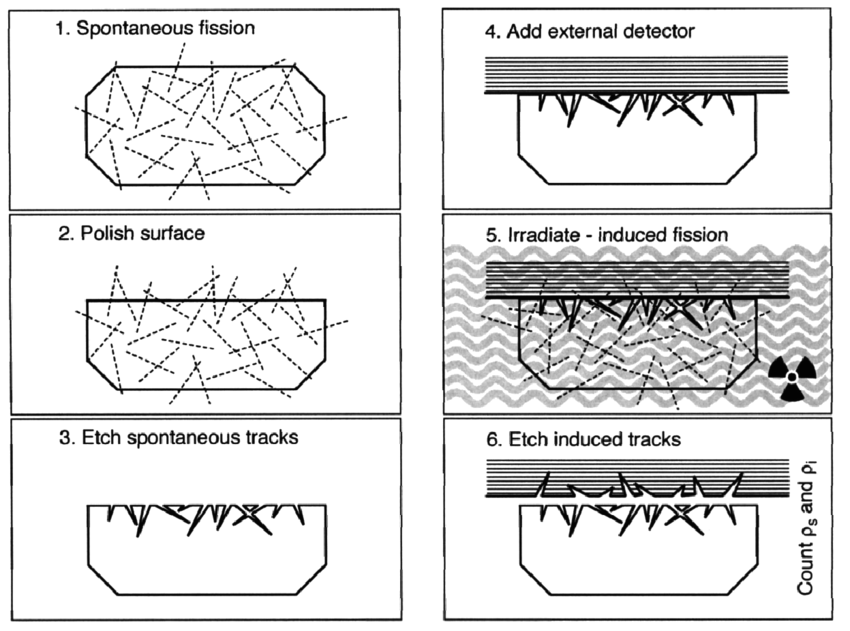
\includegraphics[width=0.8\textwidth]{fission_track.png}
    \caption{The sequence of steps involved in the external detector method of fission track dating \cite{FissionTrackDiagram}.}
    \label{fig:fission_track}
\end{figure}

\subsubsection*{Luminescence Dating}  
Luminescence dating, including optically stimulated luminescence (OSL) and thermoluminescence (TL), measures the accumulated radiation dose in minerals such as quartz and feldspar. The equivalent dose ($D_e$) is determined and used in conjunction with the dose rate ($D_r$) to calculate age:

\begin{equation}
\text{Age} = \frac{D_e}{D_r}.
\end{equation}

This method is extensively applied in Quaternary geology and archaeology to date sediments and burned materials up to several hundred thousand years old \cite{Aitken1998OSL}.
\begin{figure}[htbp]
    \centering
    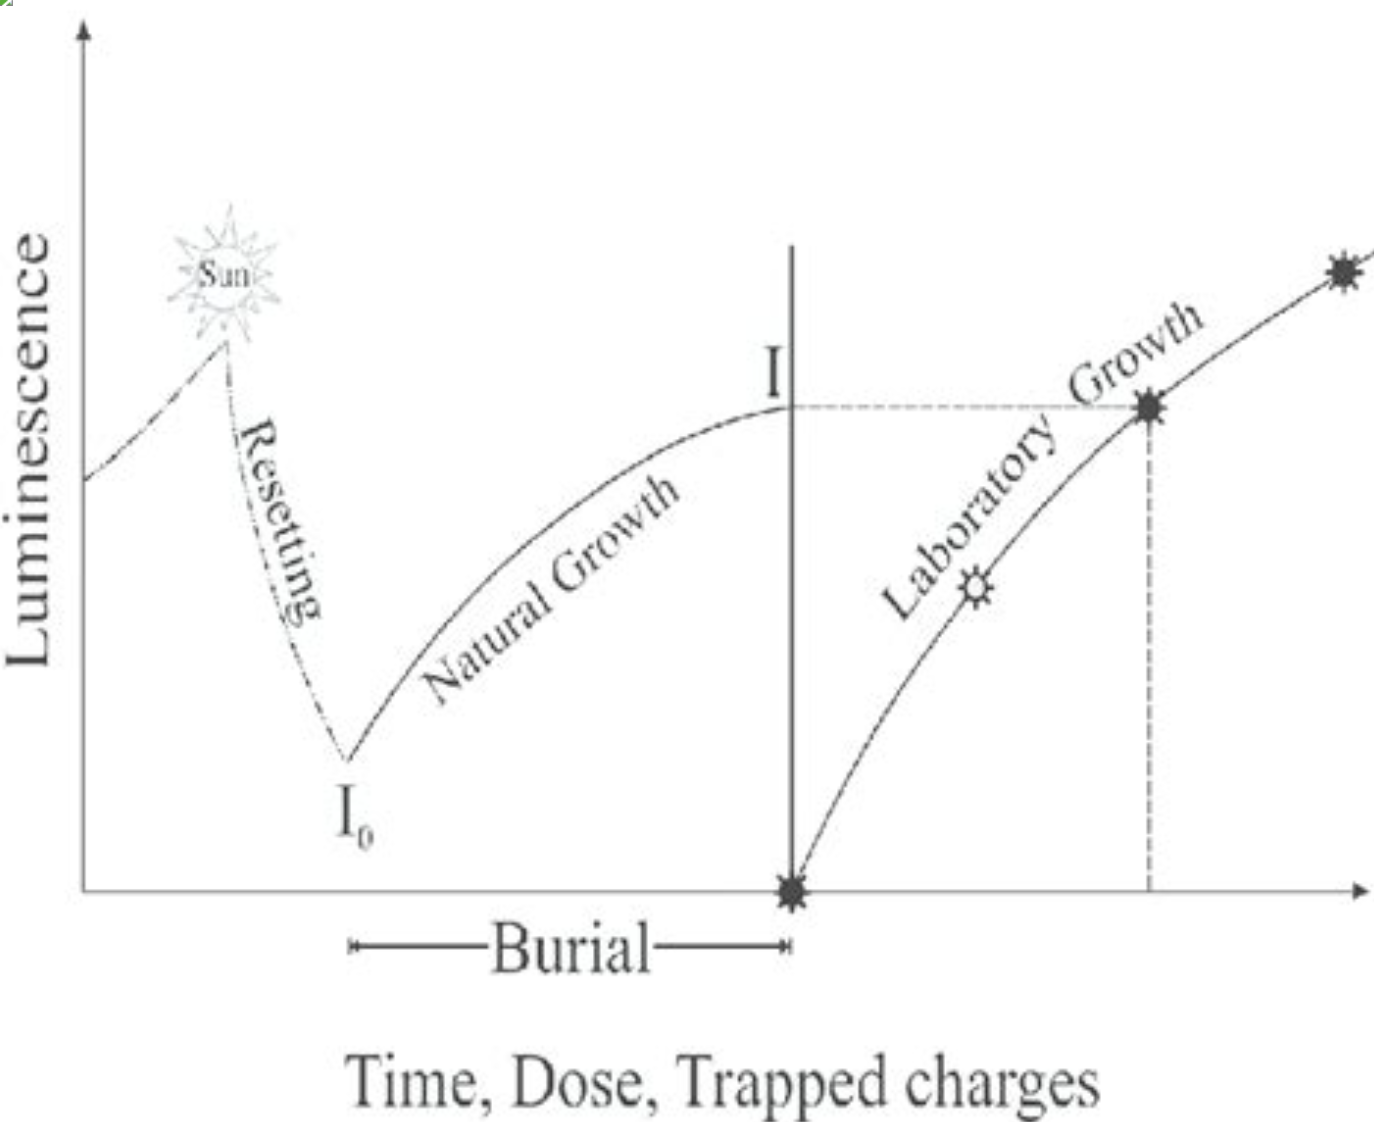
\includegraphics[width=0.8\textwidth]{luminescence_dating.png}
    \caption{Schematic diagram explaining the luminescence dating method and event chronology \cite{LuminescenceDatingDiagram}.}
    \label{fig:luminescence_dating}
\end{figure}

\subsubsection*{Future Prospects}  
With advancements in analytical techniques such as single-grain dating, laser ablation ICP-MS, and atom probe tomography, radiometric dating is becoming increasingly precise and versatile. These innovations will enhance our ability to resolve geological timescales and refine the chronology of Earth's history.

\section{Technical Principles and Methodologies}
\subsection{Isotope Analysis Instruments} \label{sec:isotope_analysis}

Isotope analysis is a fundamental aspect of radiometric dating, requiring highly precise instruments to measure isotopic ratios. The primary tools used in geochronology include thermal ionization mass spectrometry (TIMS), inductively coupled plasma mass spectrometry (ICP-MS), and laser ablation ICP-MS (LA-ICP-MS).

\subsubsection*{Thermal Ionization Mass Spectrometry (TIMS)}

TIMS is widely used for precise isotopic ratio measurements, particularly in U-Pb and Rb-Sr dating. It involves heating a sample on a filament to ionize elements, and the resulting ions are analyzed based on their mass-to-charge ratio.

The fundamental equation governing isotope decay is:

\begin{equation}
N(t) = N_0 e^{-\lambda t}
\end{equation}

where \( N(t) \) is the number of parent isotopes at time \( t \), \( N_0 \) is the initial number of parent isotopes, and \( \lambda \) is the decay constant.

TIMS offers unparalleled precision, often achieving relative errors below 0.01\%, making it indispensable for high-accuracy geochronological studies \cite{Schoene2006TIMS}.

\begin{figure}[htbp]
    \centering
    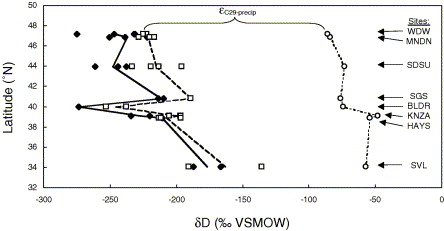
\includegraphics[width=0.75\textwidth]{Hydrogen_isotope.jpg}
    \caption{ Hydrogen isotope ratios of C29 n-alkane from C3 grasses (solid diamonds) and C4 grasses (open squares) and annual precipitation (open circles).\cite{Schoene2006TIMS}.}
    \label{fig:Hydrogen_isotope}
\end{figure}

\subsubsection*{Inductively Coupled Plasma Mass Spectrometry (ICP-MS)}

ICP-MS employs a high-temperature plasma (~10,000 K) to ionize elements before mass spectrometric analysis. This technique provides rapid analysis with excellent sensitivity, making it ideal for U-Th and Pb isotope studies.

The ion signal detected by ICP-MS follows:

\begin{equation}
I = k \cdot C \cdot \eta
\end{equation}

where \( I \) is the detected ion intensity, \( C \) is the analyte concentration, \( \eta \) is the ionization efficiency, and \( k \) is an instrument-dependent constant.

Compared to TIMS, ICP-MS enables faster sample throughput but may suffer from matrix effects and isobaric interferences, reducing precision \cite{Koornneef2014ICPMS}.



\subsubsection*{Laser Ablation ICP-MS (LA-ICP-MS)}

LA-ICP-MS integrates laser ablation with ICP-MS, enabling direct analysis of solid samples without chemical dissolution. It is widely applied in U-Pb dating of zircon \cite{Frei2009LAICPMS}.

The depth of laser penetration per pulse is given by:

\begin{equation}
d = \frac{E}{\rho \cdot H}
\end{equation}

where \( d \) is the ablation depth, \( E \) is the laser energy, \( \rho \) is the material density, and \( H \) is the heat of vaporization.


\subsubsection*{Comparison of Techniques}

Each technique has distinct advantages depending on precision, sample type, and analytical speed:

\begin{table}[htbp]
    \centering
    \caption{Comparison of TIMS, ICP-MS, and LA-ICP-MS}
    \label{tab:comparison}
    \begin{tabular}{lccc}
        \hline
        \textbf{Technique} & \textbf{Precision} & \textbf{Throughput} & \textbf{Sample Type} \\
        \hline
        TIMS & High ($<$0.01\%) & Low & Solution-based \\
        ICP-MS & Medium ($\sim$0.1\%) & High & Solution-based \\
        LA-ICP-MS & Medium ($\sim$1\%) & Very High & Solid, in-situ \\
        \hline
    \end{tabular}
\end{table}

\subsection{Sample Preparation Process}

The preparation of geological samples for radiometric dating is a critical process in obtaining reliable and accurate results. The process typically includes several stages: mineral separation, chemical dissolution, purification, and calibration with standard materials. In this section, we will describe each of these steps in detail.

\subsubsection*{Mineral Separation}

The first step in sample preparation is the separation of minerals from the collected rock samples. This separation is essential because only certain minerals, such as zircon, monazite, and feldspar, are suitable for specific types of radiometric dating. Mineral separation can be accomplished using various methods, including heavy liquid separation and magnetic separation.

Heavy liquid separation takes advantage of the density differences between minerals. Heavy liquids, such as lithium metatungstate (LST), are used to separate minerals based on whether they sink or float, depending on their density. This can be expressed as follows:

\[
\rho_{\text{mineral}} > \rho_{\text{liquid}}
\]

where \( \rho_{\text{mineral}} \) is the density of the mineral and \( \rho_{\text{liquid}} \) is the density of the liquid. If the mineral density is greater than the liquid's density, the mineral will sink. Magnetic separation, on the other hand, is useful for separating ferromagnetic minerals, such as magnetite, from non-magnetic minerals by utilizing a magnetic field.

\subsubsection*{Chemical Dissolution and Purification}

Once the minerals are separated, the next step is to dissolve the minerals and isolate the isotopes of interest. For example, zircon is typically dissolved using hydrofluoric acid (HF), which breaks down the zircon matrix but leaves uranium and thorium isotopes intact. This dissolution reaction can be written as:

\[
\text{ZrSiO}_4 (\text{solid}) + 4 \text{HF} (\text{aq}) \rightarrow \text{ZrF}_4 (\text{aq}) + 4 \text{H}_2\text{O} (\text{l}) + \text{SiF}_4 (\text{aq})
\]

Other minerals, such as feldspar, can be dissolved using hydrochloric acid (\(\text{HCl}\)). Following dissolution, the sample undergoes a purification process to remove unwanted elements such as lead and common uranium contaminants. Techniques like ion-exchange chromatography are commonly employed to separate these elements. The ion-exchange process for removing lead can be described as:

\[
\text{Pb}^{2+}_{\text{aq}} + 2 \text{Resin}_{\text{H}} \rightleftharpoons \text{Resin}_{\text{Pb}} + 2 \text{H}^+_{\text{aq}}
\]

This step ensures that only the target isotopes, such as uranium or thorium, remain in the solution for further analysis.

\subsubsection*{Calibration with Standard Materials}

Calibration is a crucial step in isotopic analysis to ensure accuracy and consistency in radiometric dating results. Primary or secondary standard materials with known isotopic compositions are used to calibrate the measurement systems. For instance, a zircon reference material with a known U-Pb isotopic composition is commonly used to calibrate mass spectrometers in U-Pb dating. This calibration process helps minimize instrumental biases, such as mass fractionation, ensuring that the measured isotopic ratios are accurate.

For U-Pb dating, the isotopic ratio of \(^{238}\text{U}\) to \(^{206}\text{Pb}\) is calibrated by comparing the sample ratio to the standard ratio, correcting for instrumental variations over time. The U-Pb ratio can be expressed as:

\[
\frac{^{238}\text{U}}{^{206}\text{Pb}} = e^{\lambda_{\text{U238}} t} - 1
\]

where \( \lambda_{\text{U238}} \) is the decay constant for \(^{238}\text{U}\) and \( t \) is the time elapsed since the last reset event, such as crystallization or metamorphism.

\subsubsection*{Challenges in Sample Preparation}

Despite advances in sample preparation techniques, challenges remain. Contamination from environmental sources, such as modern carbon in \(^{14}\text{C}\) dating or atmospheric contamination in U-Pb dating, can significantly alter the isotopic ratios \cite{Dodson1973}. To mitigate contamination, samples are processed under strict protocols in cleanroom environments, and inert gas atmospheres are used for handling sensitive samples.

Isotopic fractionation—when isotopes behave differently during chemical or physical processes—can also lead to errors. For instance, lighter isotopes of uranium may dissolve more readily than heavier isotopes during the dissolution process, causing a deviation from the expected isotopic ratios. This fractionation is corrected by applying known models based on isotope behavior during chemical processes \cite{Rutherford2002}.

\begin{figure}[htbp]
    \centering
    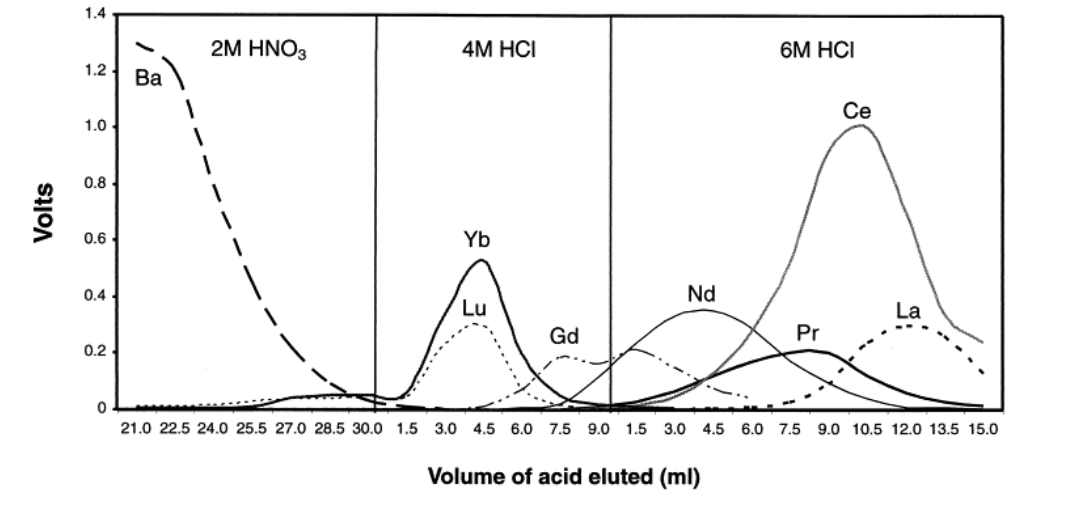
\includegraphics[width=0.75\textwidth]{Chemical_process.png}
    \caption{Chemical process:cation exchange separation).\cite{Rutherford2002}.}
    \label{fig:Chemical_process}
\end{figure}

In U-Pb dating, the fractionation correction can be applied using the following equation:

\[
\left(\frac{^{238}\text{U}}{^{206}\text{Pb}}\right)_{\text{corrected}} = \left(\frac{^{238}\text{U}}{^{206}\text{Pb}}\right)_{\text{measured}} \times \left(1 + \alpha_{\text{U-Pb}} \times \Delta T\right)
\]

where \( \alpha_{\text{U-Pb}} \) is the isotopic fractionation factor, and \( \Delta T \) represents the temperature deviation during sample preparation.

\subsubsection*{Example: U-Pb Dating of Zircon}

As an example, the procedure for U-Pb dating of zircon involves isolating zircon crystals from a rock sample, dissolving them in HF, purifying the sample, and measuring the isotopic ratio using mass spectrometry. The age is then determined using the equation for the U-Pb system, where the age \( t \) is calculated from the measured ratio of \(^{238}\text{U}\) to \(^{206}\text{Pb}\):

\[
\frac{^{238}\text{U}}{^{206}\text{Pb}} = e^{\lambda_{\text{U238}} t} - 1
\]

By measuring the isotopic ratio, the age of the sample can be determined with high precision.

\subsection{Data Processing and Sources of Uncertainty}

Accurate geochronological interpretations require robust data processing techniques to derive reliable ages from isotopic measurements. The fundamental goal is to translate raw isotopic ratios into meaningful geological ages while accounting for analytical and natural sources of uncertainty. This section discusses key age calculation models, common sources of error, and statistical methods used to quantify uncertainty in radiometric dating.

\subsubsection*{Age Calculation Models}

Radiometric dating relies on solving the fundamental decay equation:

\[
N(t) = N_0 e^{-\lambda t}
\]

where:
- \( N(t) \) is the number of radioactive parent isotopes remaining at time \( t \),
- \( N_0 \) is the initial number of parent isotopes,
- \( \lambda \) is the decay constant (\(\lambda = \frac{\ln 2}{T_{1/2}}\), where \(T_{1/2}\) is the half-life),
- \( t \) is the time elapsed since the system was closed.

For isotopic systems such as U-Pb, age calculations are often derived from isotope ratio measurements rather than absolute atom counts. The Pb/U ratio provides a direct means of computing age using the following relations:

\[
^{206}\text{Pb}/^{238}\text{U} = e^{\lambda_{238} t} - 1
\]

\[
^{207}\text{Pb}/^{235}\text{U} = e^{\lambda_{235} t} - 1
\]

The Concordia diagram, introduced by Wetherill \cite{Wetherill1956}, plots these two ratios against each other, where the intersection of the measured data with the Concordia curve provides an estimate of sample age.

Similarly, in isochron dating (e.g., Rb-Sr and Sm-Nd methods), the age is derived from the equation:

\[
^{87}\text{Sr}/^{86}\text{Sr} = \left( \frac{^{87}\text{Rb}}{^{86}\text{Sr}} \right) (e^{\lambda t} - 1) + \left( \frac{^{87}\text{Sr}}{^{86}\text{Sr}} \right)_{\text{initial}}
\]

which represents a straight-line equation in an isochron diagram, where the slope \( m = e^{\lambda t} - 1 \) yields the sample's age.

\subsubsection*{Sources of Analytical Uncertainty}

Uncertainty in radiometric dating arises from multiple factors, including instrumental precision, sample contamination, and assumptions about system closure. Common sources of error include:

\begin{itemize}
    \item \textbf{Instrumental noise:} Mass spectrometric techniques such as TIMS and ICP-MS introduce uncertainties due to detector precision, electronic noise, and ion counting statistics \cite{Rutherford2002}.
    \item \textbf{Fractionation effects:} Isotope fractionation during sample processing can alter measured isotopic ratios. Mass-dependent fractionation follows the power-law relation:

    \[
    \frac{R_{\text{measured}}}{R_{\text{true}}} = \left( \frac{m_1}{m_2} \right)^\beta
    \]

    where \( m_1 \) and \( m_2 \) are isotope masses, and \( \beta \) is an empirically determined exponent.
    \item \textbf{Initial daughter isotopes:} In systems like Rb-Sr dating, the presence of initial \(^{87}\)Sr can skew calculated ages, necessitating isochron methods to resolve inherited components.
    \item \textbf{Open-system behavior:} Diffusive loss of daughter isotopes due to thermal events can alter age calculations. Closure temperature models \cite{Dodson1973} define the temperature at which isotopic diffusion ceases:

    \[
    T_c = \frac{E_a}{R \ln \left( \frac{A D_0}{r^2 \lambda} \right)}
    \]

    where:
    - \( T_c \) is the closure temperature,
    - \( E_a \) is the activation energy for diffusion,
    - \( R \) is the gas constant,
    - \( A \) is a geometric factor,
    - \( D_0 \) is the diffusion coefficient at infinite temperature,
    - \( r \) is the effective diffusion radius.

\end{itemize}

\begin{figure}[htbp]
    \centering
    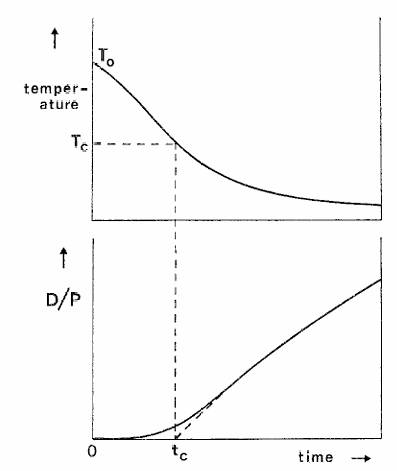
\includegraphics[width=0.75\textwidth]{Closure_temp.png}
    \caption{Closeure temperature definition.\cite{Dodson1973}.}
    \label{fig:Closure_temp}
\end{figure}

\subsubsection*{Error Propagation and Uncertainty Quantification}

Uncertainty in age determination propagates from multiple sources, including isotopic ratio measurements and decay constants. The total uncertainty (\(\sigma_t\)) can be estimated using error propagation:

\[
\sigma_t^2 = \left( \frac{\partial t}{\partial R} \sigma_R \right)^2 + \left( \frac{\partial t}{\partial \lambda} \sigma_\lambda \right)^2
\]

where:
- \( R \) is the isotopic ratio,
- \( \sigma_R \) is the uncertainty in the ratio measurement,
- \( \sigma_\lambda \) is the uncertainty in the decay constant.

For Concordia-based U-Pb dating, Monte Carlo simulations and Bayesian statistics are often employed to refine uncertainty estimates and correct for discordance caused by Pb loss.

\subsubsection*{Best Practices in Data Interpretation}

To ensure accuracy and reproducibility in geochronology, several best practices should be followed:

\begin{itemize}
    \item Use well-characterized standard materials to calibrate isotope measurements.
    \item Employ multiple dating methods on the same sample to cross-validate ages.
    \item Consider geological context, as metamorphic overprints can reset isotopic systems.
    \item Apply numerical modeling (e.g., diffusion kinetics) to assess potential post-crystallization isotope mobility.
\end{itemize}

By integrating rigorous data processing techniques with error analysis, radiometric dating continues to provide precise and reliable constraints on Earth's geological history.

\section{Case Studies in Geochronology}
\subsection{Archean Crustal Evolution: U-Pb and Lu-Hf Insights from the Acasta Gneiss Complex}
\label{subsec:acasta_case}

The Acasta Gneiss Complex (AGC) in northwestern Canada preserves Earth's oldest known crustal fragments, providing critical constraints on Hadean to Paleoarchean geodynamics. This case study integrates U-Pb zircon chronology with Lu-Hf isotope systematics to unravel early continental growth mechanisms.

\subsubsection*{Geological Context and Sample Selection}
The AGC comprises polyphase orthogneisses dated between 4.03-3.94 Ga \cite{Bowring1999}. Key sampling criteria include:
\begin{itemize}
    \item Preservation of igneous zircon domains (CL-bright, sector-zoned)
    \item Absence of secondary Pb-loss (Th/U < 0.1 in altered zones)
    \item Coherence with regional structural trends (NW-SE foliation)
\end{itemize}

\subsubsection*{Analytical Approach}
\begin{enumerate}
    \item \textbf{U-Pb ID-TIMS Dating}:  
    High-precision analyses used the EARTHTIME \(^{202}\text{Pb}\)-\(^{205}\text{Pb}\)-\(^{233}\text{U}\)-\(^{235}\text{U}\) tracer:
    \begin{equation}
        \left(\frac{^{207}\text{Pb}}{^{206}\text{Pb}}\right)_{\text{meas}} = \left(\frac{^{235}\text{U}}{^{238}\text{U}}\right)_{\text{init}} \frac{e^{\lambda_{235}t} - 1}{e^{\lambda_{238}t} - 1}
        \label{eq:pb_pb}
    \end{equation}
    with \(\lambda_{235} = 9.8485 \times 10^{-10}\ \text{yr}^{-1}\) \cite{Jaffey1975}.

    \item \textbf{Lu-Hf MC-ICPMS}:  
    Measured \(^{176}\text{Hf}/^{177}\text{Hf}\) ratios converted to \(\epsilon_{\text{Hf}}\) values:
    \begin{equation}
        \epsilon_{\text{Hf}} = \left[\frac{(^{176}\text{Hf}/^{177}\text{Hf})_{\text{sample}}}{(^{176}\text{Hf}/^{177}\text{Hf})_{\text{CHUR}}} - 1\right] \times 10^4
        \label{eq:ehf}
    \end{equation}
    where CHUR = 0.282785.
\end{enumerate}

\subsubsection*{Results and Interpretation}
\begin{itemize}
    \item \textbf{Oldest Crystallization Ages}:  
    ID-TIMS analyses yield concordant ages up to \(4016 \pm 8\ \text{Ma}\) (MSWD = 0.98), defining the AGC basement (Fig. \ref{fig:acasta_concordia}).

    \item \textbf{Hf Isotope Evolution}:  
    Initial \(\epsilon_{\text{Hf}}\) values range from \(-2.1\) to \(+1.3\), straddling chondritic evolution (Fig. \ref{fig:hf_evolution}). This implies:
    \begin{equation}
        f_{\text{Lu/Hf}} = \left(\frac{^{176}\text{Lu}/^{177}\text{Hf}}{^{176}\text{Lu}/^{177}\text{Hf}_{\text{CHUR}}}\right) - 1 \approx 0.03\--0.12
        \label{eq:f_luhf}
    \end{equation}
    indicative of juvenile crustal growth \cite{Vervoort2015}.

    \item \textbf{Tectonic Implications}:  
    The combined U-Pb-Hf dataset supports a model of:
    \begin{itemize}
        \item Episodic crustal extraction from depleted mantle (DM) at 4.0-3.9 Ga
        \item Re-working through Eoarchean convergent tectonics
        \item Limited early crustal differentiation (\(<10\%\) felsic component)
    \end{itemize}
\end{itemize}

\begin{figure}[htbp]
    \centering
    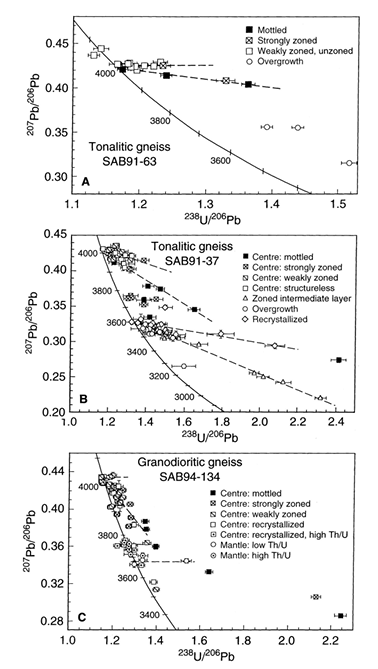
\includegraphics[width=0.75\textwidth]{acasta_concordia.png}
    \caption{Concordia diagram for ID-TIMS analyses of Acasta zircon. Error ellipses at 2\(\sigma\). Data from \cite{Bowring1999}.}
    \label{fig:acasta_concordia}
\end{figure}

\begin{figure}[htbp]
    \centering
    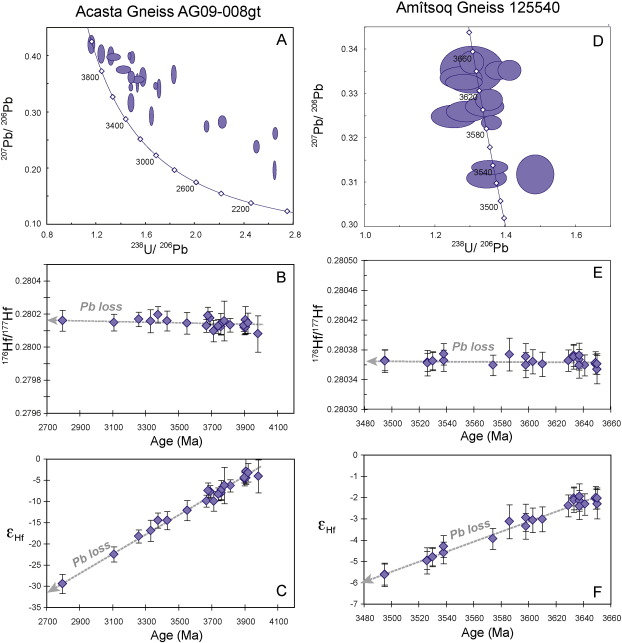
\includegraphics[width=0.75\textwidth]{hf_evolution.jpg}
    \caption{Lu-Hf isotope evolution diagram for AGC samples. DM = Depleted Mantle. After \cite{Vervoort2015}.}
    \label{fig:hf_evolution}
\end{figure}


\subsection{Quaternary Climate Cycles: \(^{230}\text{Th}/^{238}\text{U}\) Speleothem Chronology of the Asian Monsoon}
\label{subsec:monsoon_case}

Speleothems (cave deposits) provide unparalleled archives of Quaternary climate variability through their \(^{230}\text{Th}/^{238}\text{U}\) chronologies coupled with \(\delta^{18}\text{O}\) proxies. This case study focuses on the Hulu Cave record (China), which has redefined our understanding of Dansgaard-Oeschger (D-O) events during the last glacial period.

\subsubsection*{Speleothem Formation Dynamics}
The \(^{230}\text{Th}/^{238}\text{U}\) dating method relies on:
\begin{itemize}
    \item Initial \(^{230}\text{Th} = 0\) assumption (closed-system carbonate precipitation)
    \item Constant dripwater \(^{238}\text{U}\) concentration
    \item High U content (0.1-10 ppm) for precise measurement
\end{itemize}

The age equation is derived from radioactive decay:
\begin{equation}
    t = \frac{1}{\lambda_{230}} \ln\left(1 + \frac{{}^{230}\text{Th}}{{}^{238}\text{U}} \left(1 - e^{-\lambda_{234}t}\right) + \frac{\delta^{234}\text{U}}{1000}\right)
    \label{eq:thu_age}
\end{equation}
where \(\lambda_{230} = 9.158 \times 10^{-6}\ \text{yr}^{-1}\) and \(\delta^{234}\text{U}\) initial value \cite{Cheng2013}.

\subsubsection*{Analytical Protocol}
\begin{enumerate}
    \item \textbf{Sample Preparation}:  
    - Micromill 100-200 mg calcite along growth axis  
    - Chemical separation using Eichrom UTEVA resins
    
    \item \textbf{MC-ICPMS Analysis}:  
    Achieve 0.1-0.5\% precision (2\(\sigma\)) via \(^{229}\text{Th}\)-\(^{233}\text{U}\)-\(^{236}\text{U}\) triple spike:
    \begin{equation}
        \left(\frac{{}^{230}\text{Th}}{{}^{238}\text{U}}\right)_{\text{corr}} = \left(\frac{{}^{230}\text{Th}}{{}^{238}\text{U}}\right)_{\text{meas}} \times \left(1 + \frac{\epsilon_{\text{spike}}}{10^4}\right)
        \label{eq:spike_corr}
    \end{equation}
    
    \item \textbf{Age Model Construction}:  
    Bayesian interpolation (Bacon software) with:
    \begin{equation}
        \text{MSWD} = \frac{1}{n-1}\sum_{i=1}^n \left(\frac{t_i - \hat{t}_i}{\sigma_i}\right)^2 < 1.5
        \label{eq:mswd}
    \end{equation}
\end{enumerate}

\subsubsection*{Hulu Cave D-O Event Chronology}
\begin{itemize}
    \item \textbf{Timing Precision}:  
    D-O 12 onset dated to \(44.7 \pm 0.3\ \text{ka BP}\) (Fig. \ref{fig:d_o_curve}), synchronizing with Greenland ice cores within 50 years \cite{Wang2001}.
    
    \item \textbf{Monsoon-AMOC Linkage}:  
    Cross-correlation shows:
    \begin{equation}
        r(\tau) = \frac{\int \delta^{18}\text{O}_{\text{Hulu}}(t) \cdot \delta^{18}\text{O}_{\text{GRIP}}(t+\tau) dt}{\sqrt{\int \delta^{18}\text{O}_{\text{Hulu}}^2 dt \cdot \int \delta^{18}\text{O}_{\text{GRIP}}^2 dt}} = 0.82\ (\tau = -12\ \text{yr})
        \label{eq:correlation}
    \end{equation}
    indicating Asian monsoon leads Atlantic circulation changes \cite{Cheng2016}.
\end{itemize}

\subsubsection*{Implications for Climate Forcing}
The \(^{230}\text{Th}/^{238}\text{U}\)-dated record demonstrates:
\begin{itemize}
    \item Solar insolation control on monsoon intensity at precessional (23-kyr) bands
    \item Heinrich stadial triggers for megadroughts
    \item Bipolar seesaw dynamics resolved to centennial scale
\end{itemize}

\begin{figure}[htbp]
    \centering
    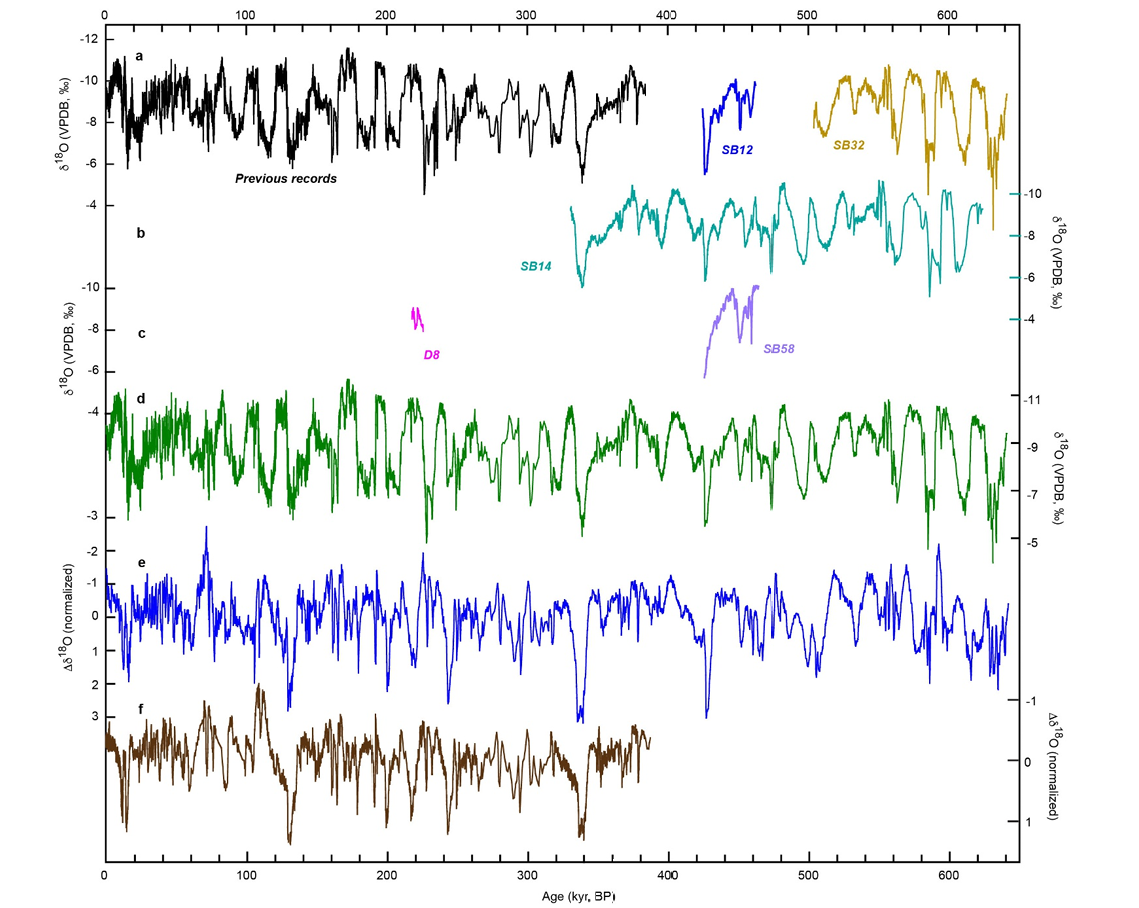
\includegraphics[width=0.85\textwidth]{hulu_dansgaard.png}
    \caption{Hulu Cave \(\delta^{18}\text{O}\) record (red) versus NGRIP ice core (blue). Vertical bars mark D-O events. Data from \cite{Cheng2016}.}
    \label{fig:d_o_curve}
\end{figure}

 \subsection{Martian Chronology: \(^{40}\text{Ar}/^{39}\text{Ar}\) Dating of Shergottite Meteorites}
\label{subsec:martian_case}

Shergottite meteorites provide critical constraints on the volcanic and impact history of Mars. This study focuses on Northwest Africa (NWA) 7034 "Black Beauty" — a polymict breccia containing the oldest known Martian zircons — using \(^{40}\text{Ar}/^{39}\text{Ar}\) step-heating and U-Pb CA-ID-TIMS analyses.

\subsubsection*{Sample Characteristics and Preparation}
\begin{itemize}
    \item \textbf{Breccia Components}:  
    - 4.4 Ga zircon clasts (ID-TIMS U-Pb) \cite{Humayun2013}  
    - 1.5 Ga basaltic matrix (Ar-Ar plateau ages)  
    - Impact melt glasses (0.2-0.7 Ga)
    
    \item \textbf{Mineral Separation}:  
    - Crushing under Ar atmosphere (<1 ppm terrestrial contamination)  
    - Density separation (zircon: \(\rho > 4.6\ \text{g/cm}^3\))  
    - Hand-picking under binocular microscope
\end{itemize}

\subsubsection*{\(^{40}\text{Ar}/^{39}\text{Ar}\) Step-Heating Protocol}
\begin{enumerate}
    \item \textbf{Neutron Irradiation}:  
    Cadmium-shielded irradiation for \(J = 0.00125 \pm 0.00003\) (Fish Canyon sanidine monitor)
    
    \item \textbf{Stepwise Degassing}:  
    15 temperature steps from 500°C to 1600°C, with gas cleanup using SAES GP-50 getters
    
    \item \textbf{Isotope Ratio Calculation}:  
    Corrected for cosmogenic \(^{36}\text{Ar}\):
    \begin{equation}
        \left(\frac{{}^{40}\text{Ar}}{{}^{39}\text{Ar}}\right)_{\text{corr}} = \left(\frac{{}^{40}\text{Ar}}{{}^{39}\text{Ar}}\right)_{\text{meas}} - 0.65\left(\frac{{}^{36}\text{Ar}}{{}^{39}\text{Ar}}\right)
        \label{eq:cosmo_corr}
    \end{equation}
\end{enumerate}

\subsubsection*{Age Interpretation Framework}
The inverse isochron age is calculated via:
\begin{equation}
    \left(\frac{{}^{40}\text{Ar}}{{}^{36}\text{Ar}}\right) = \left(\frac{{}^{40}\text{Ar}}{{}^{36}\text{Ar}}\right)_{\text{initial}} + \left(\frac{{}^{39}\text{Ar}}{{}^{36}\text{Ar}}\right)\left(e^{\lambda t} - 1\right)J
    \label{eq:inverse_isochron}
\end{equation}

For NWA 7034 matrix material:
\begin{itemize}
    \item Plateau age: \(1472 \pm 14\ \text{Ma}\) (MSWD = 1.3, 68\% \(^{39}\text{Ar}\) release)  
    \item Initial \(^{40}\text{Ar}/^{36}\text{Ar} = 275 \pm 18\) (Martian atmosphere signature)
\end{itemize}

\subsubsection*{Impact Chronology Constraints}
Combined U-Pb/Ar-Ar data reveal:
\begin{itemize}
    \item Major impact at \(4.43 \pm 0.03\ \text{Ga}\) (zircon shock features)  
    \item Amazonian resurfacing events at \(1.47\ \text{Ga}\) and \(615\ \text{Ma}\)  
    \item Martian mantle differentiation age: \(4.53\ \text{Ga}\) via \(^{182}\text{Hf}\)-\(^{182}\text{W}\) \cite{Kleine2009}
\end{itemize}

\subsection{Thermochronology of Orogenic Belts: Fission-Track Dating in the Himalayas}
\label{subsec:fission_track_case}

Fission-track thermochronology provides unique insights into the exhumation and thermal evolution of collisional orogens. This case study focuses on the eastern Himalayan syntaxis, combining zircon (ZFT) and apatite (AFT) fission-track analyses to constrain the Miocene-Pliocene uplift history.

\subsubsection*{Fission-Track Fundamentals}
The method relies on spontaneous fission of \(^{238}\text{U}\) producing latent tracks in crystal lattices. The age equation incorporates both decay and track annealing:
\begin{equation}
    t = \frac{1}{\lambda_d} \ln\left(1 + \frac{\lambda_d \rho_s}{\lambda_f \rho_i} G \right)
    \label{eq:ft_age}
\end{equation}
where:
\begin{itemize}
    \item \(\lambda_d = 1.55125 \times 10^{-10}\ \text{yr}^{-1}\) (total decay constant)
    \item \(\lambda_f = 8.46 \times 10^{-17}\ \text{yr}^{-1}\) (spontaneous fission constant)
    \item \(G\): Geometry factor (0.5 for external detector method)
\end{itemize}

\subsubsection*{Analytical Workflow}
\begin{enumerate}
    \item \textbf{Mineral Separation}:  
    - Heavy liquid separation (\(\rho = 3.3-3.5\ \text{g/cm}^3\) for apatite)  
    - Epoxy mounting and polishing to 0.25 μm finish
    
    \item \textbf{Irradiation and Etching}:  
    - Cd-lined irradiation (\(10^{15}\ \text{n/cm}^2\)) to induce \(^{235}\text{U}\) fission  
    - 5.5M HNO\(_3\) (20°C, 20s) for apatite track revelation
    
    \item \textbf{Automated Microscopy}:  
    Use of FastTrackscan software with CNN-based track recognition:
    \begin{equation}
        \text{Accuracy} = \frac{\text{TP}}{\text{TP} + \text{FP} + \text{FN}} > 95\% 
        \label{eq:cnn_acc}
    \end{equation}
    where TP=True Positives, FP=False Positives \cite{Gleadow2015}
\end{enumerate}

\subsubsection*{Himalayan Exhumation Phases}
\begin{itemize}
    \item \textbf{ZFT Data (24-15 Ma)}:  
    - Records initial crustal thickening:  
    \begin{equation}
        \frac{dT}{dt} = 15-25^\circ \text{C/Myr} \quad (P = 0.8-1.2\ \text{GPa})
        \label{eq:zft_cooling}
    \end{equation}
    
    \item \textbf{AFT Data (10-2 Ma)}:  
    - Reveals late-stage rapid exhumation:  
    \begin{equation}
        \text{Exhumation Rate} = \frac{\Delta z}{\Delta t} = 2.5-3.8\ \text{mm/yr}
        \label{eq:exhum_rate}
    \end{equation}
    
    \item \textbf{Thermal Modeling}:  
    HeFTy simulations yield two-stage cooling history (Fig. \ref{fig:hefty}):
    \begin{itemize}
        \item Stage I (20-10 Ma): Thrust wedge underplating  
        \item Stage II (<5 Ma): River incision-dominated
    \end{itemize}
\end{itemize}

\subsubsection*{Tectonic Implications}
\begin{itemize}
    \item Coupling between surface processes and crustal flow  
    \item Partitioning of strain across Himalayan frontal thrust  
    \item Climate-tectonic feedback via monsoon intensification
\end{itemize}

\begin{figure}[htbp]
    \centering
    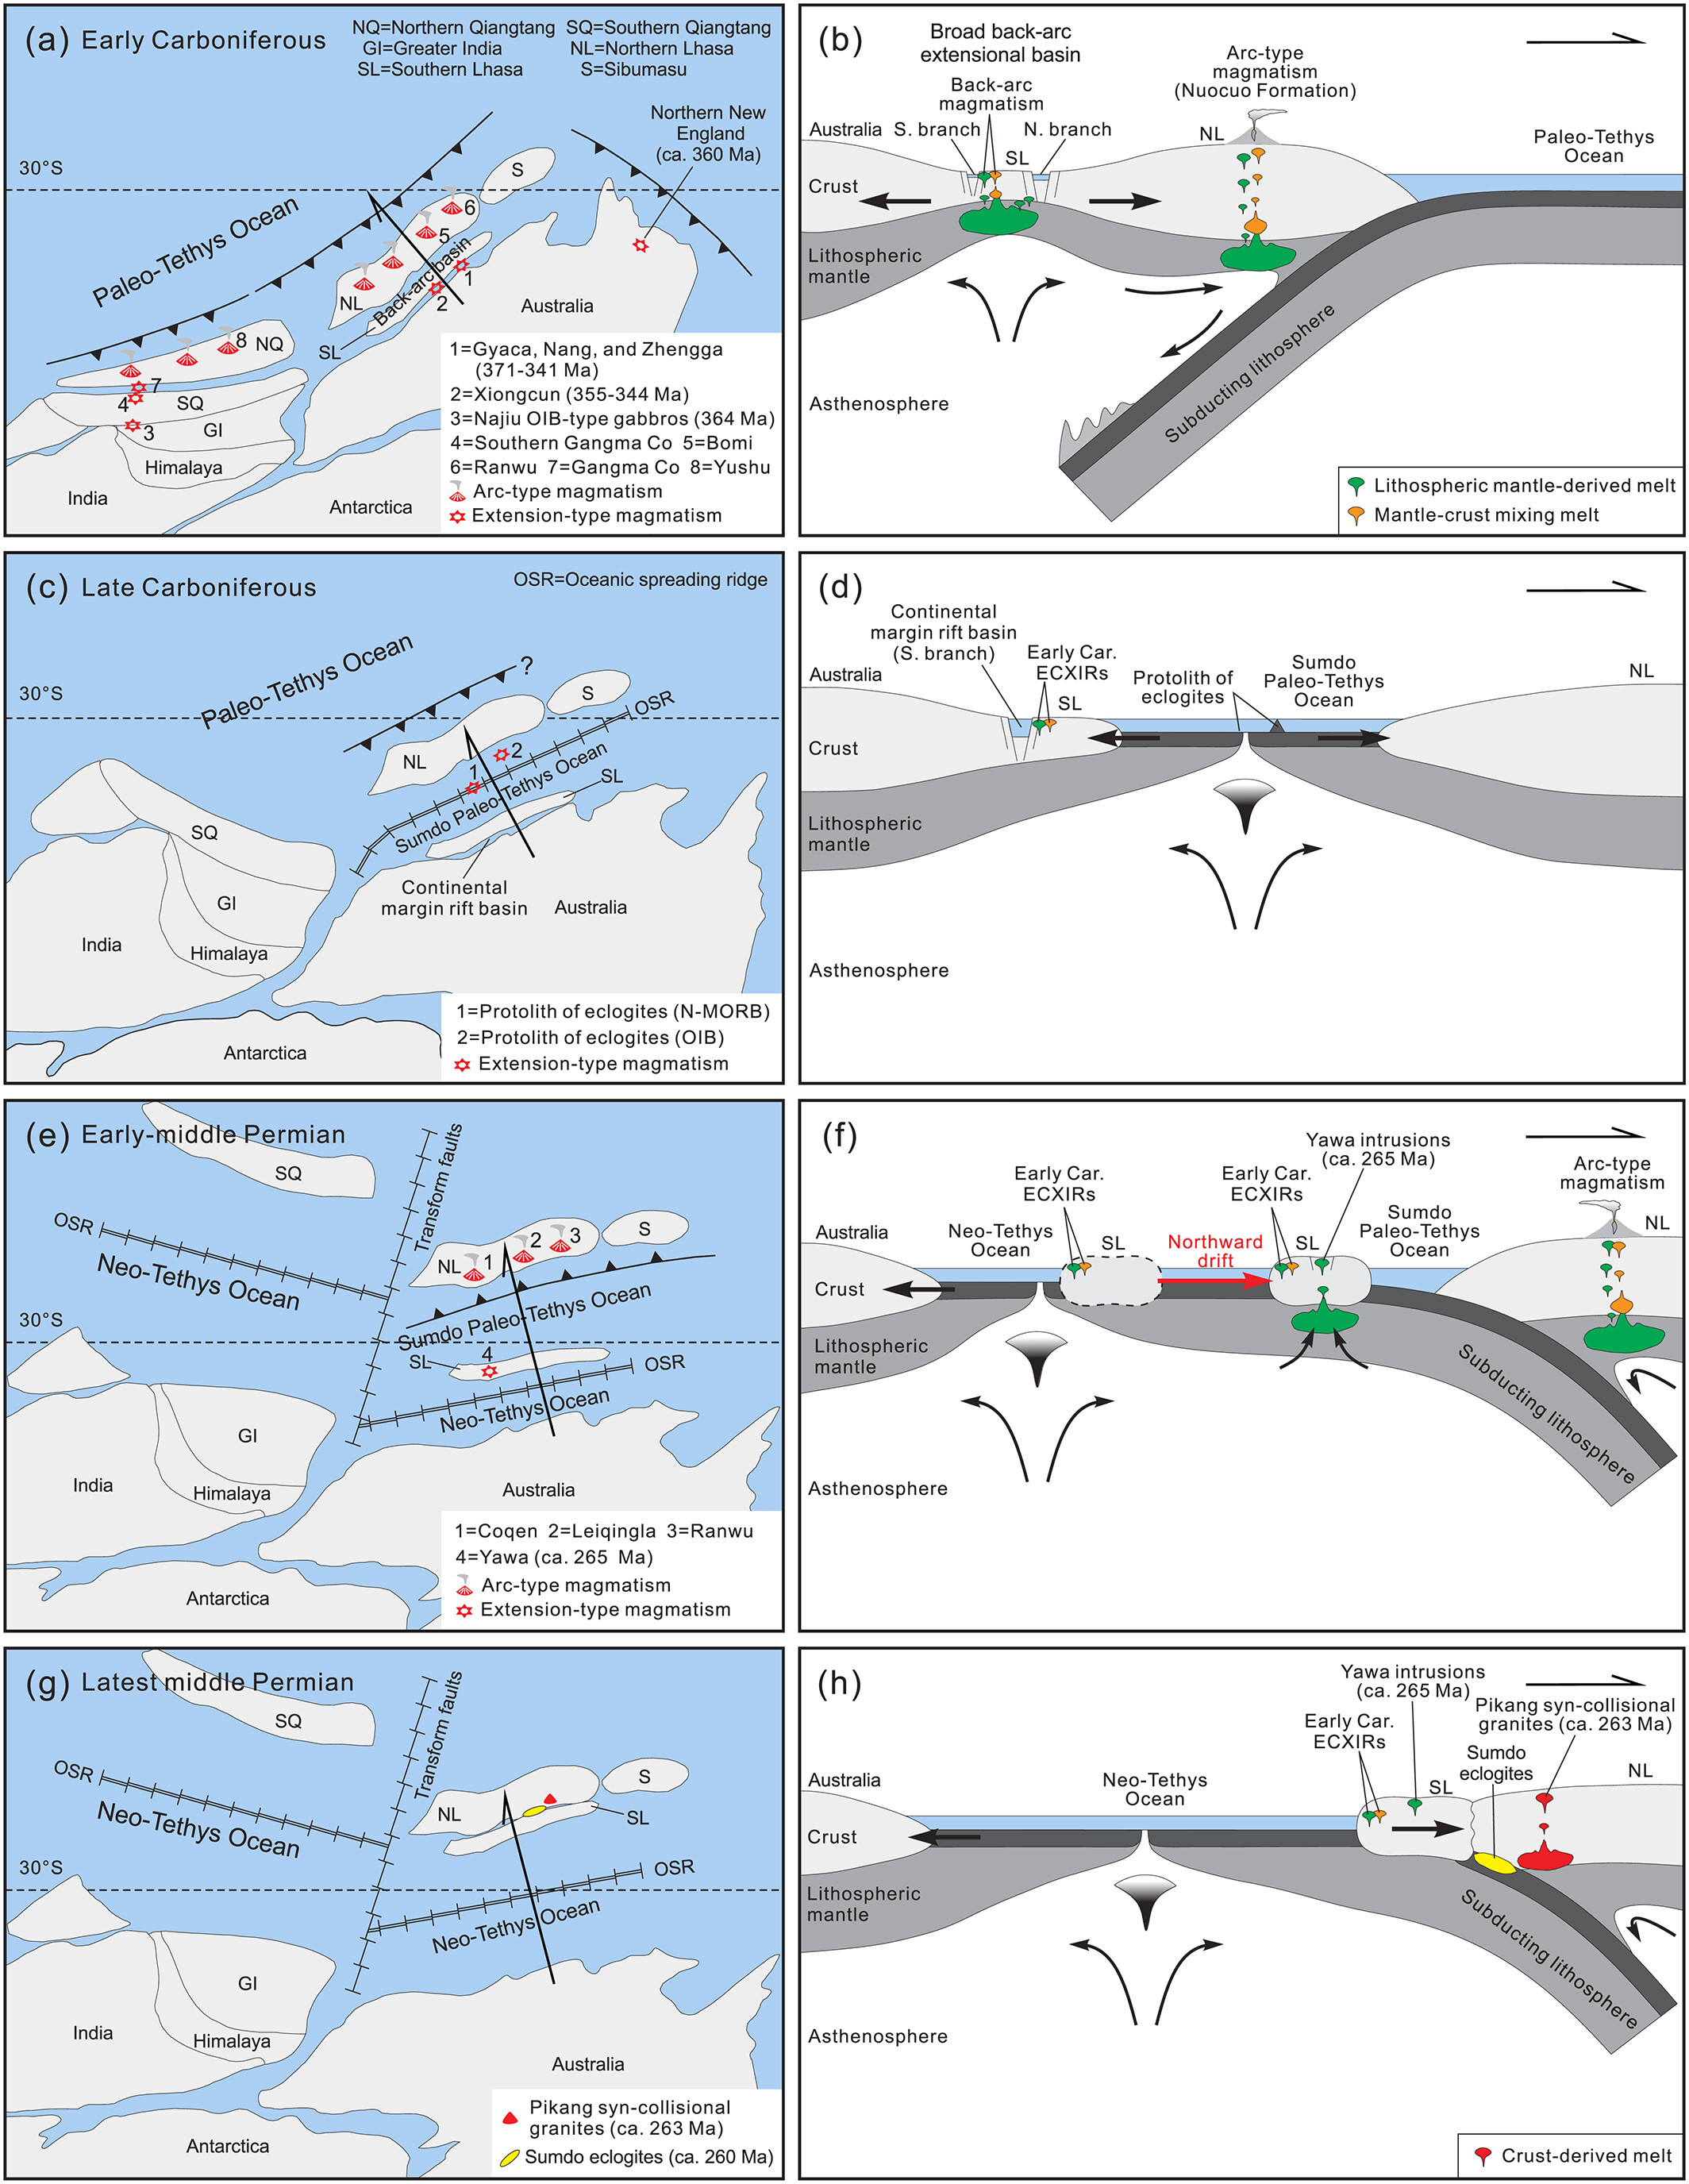
\includegraphics[width=0.85\textwidth]{hefty_plot.jpg}
    \caption{Time-temperature paths from inverse modeling of ZFT and AFT data. Shaded regions show 95\% confidence intervals. Modified from \cite{King2020}.}
    \label{fig:hefty}
\end{figure}

\section{Challenges and Future Directions}
\subsection{Technical Limitations in Radiometric Dating Systems}
\label{subsec:challenges}

Despite significant advancements, radiometric dating methods face persistent technical challenges that limit their accuracy and applicability. This section critically examines four major limitations across different isotopic systems.

\subsubsection*{1. Radiation Damage Effects in U-Pb Zircon Dating}
Metamictization caused by \(\alpha\)-decay of U and Th damages zircon lattices, leading to Pb loss and discordant ages. The radiation dose (\(D\)) is quantified as:
\begin{equation}
    D = N_{\text{U}} \cdot (1 + 0.235 \cdot \text{Th/U}) \cdot t \cdot \lambda_{\alpha}
    \label{eq:radiation_dose}
\end{equation}
where \(N_{\text{U}}\) is U concentration (ppm), \(t\) age (Ma), \(\lambda_{\alpha} = 1.551 \times 10^{-10}\ \text{yr}^{-1}\). Critical damage threshold occurs at \(D \approx 5 \times 10^{18}\ \alpha/\text{g}\) \cite{Nasdala2001}.

\subsubsection*{2. Argon Redistribution in K-Ar Systems}
In \(^{40}\text{Ar}/^{39}\text{Ar}\) dating, sub-grain scale Ar mobility produces "staircase" age spectra. The effective diffusion radius (\(r_{\text{eff}}\)) follows:
\begin{equation}
    \frac{\partial C}{\partial t} = D_0 \exp\left(-\frac{E_a}{RT}\right) \nabla^2 C
    \label{eq:arg_diffusion}
\end{equation}
where \(C\) is Ar concentration, \(D_0\) pre-exponential factor (\(10^{-3}\ \text{cm}^2/\text{s}\) for feldspar). Sub-micron domains yield apparent ages <1\% precision \cite{Villa2016}.

\subsubsection*{3. Carbon Reservoir Effects in \(^{14}\text{C}\) Dating}
Marine reservoir corrections require precise \(\Delta R\) determination:
\begin{equation}
    \Delta R = R_{\text{local}} - R_{\text{global}} = \frac{{}^{14}\text{C}_{\text{atm}} - {}^{14}\text{C}_{\text{marine}}}{\lambda}
    \label{eq:delta_r}
\end{equation}
Uncertainties in pre-bomb \(\Delta R\) values (\(\pm 50-150\ \text{yr}\)) limit coastal archaeology dating \cite{Reimer2020}.

\subsubsection*{4. Interlaboratory Calibration Discrepancies}
Between-lab bias persists due to standard heterogeneity. For zircon standards (TEMORA 2):
\begin{equation}
    \text{Reproducibility} = \sqrt{\frac{\sum_{i=1}^n (x_i - \bar{x})^2}{n-1}} = 0.3-0.8\%\ (2\sigma)
    \label{eq:reproducibility}
\end{equation}
exceeding ideal <0.1\% requirements.

\subsection{Cross-Disciplinary Integration}

The integration of geochronological methods with other scientific disciplines has become increasingly essential for improving the precision and scope of radiometric dating techniques. In this section, we will discuss several key cross-disciplinary integrations in the context of geological, archaeological, and climate studies. These interdisciplinary approaches enhance both the reliability and the interpretive power of radiometric data.

\subsubsection*{Geochronology and Climate Science}

One of the most significant applications of cross-disciplinary integration is in the reconstruction of past climates. By combining radiometric dating techniques with geochemical tracers, scientists can establish precise timelines of climate events. Oxygen isotopes in carbonate minerals are commonly used to reconstruct past temperatures, with the ratio of \(^{18}\text{O}/^{16}\text{O}\) providing a reliable temperature proxy.

For example, the use of U-Th dating on coral reefs or stalagmites, in combination with oxygen isotope analysis, has enabled the reconstruction of past sea levels and temperature fluctuations during the Holocene. The governing equation for U-Th dating is given by:

\begin{equation}
\frac{^{230}\text{Th}}{^{234}\text{U}} = \frac{^{230}\text{Th}_0}{^{234}\text{U}_0} e^{-\lambda_U t} - e^{-\lambda_{\text{Th}} t}
\end{equation}

where \( t \) represents the time elapsed since the sample was last reset, and \(\lambda_U\) and \(\lambda_{\text{Th}}\) are the decay constants of Uranium and Thorium. This integration provides robust data for reconstructing past climate and sea-level changes.

\begin{figure}
    \centering
    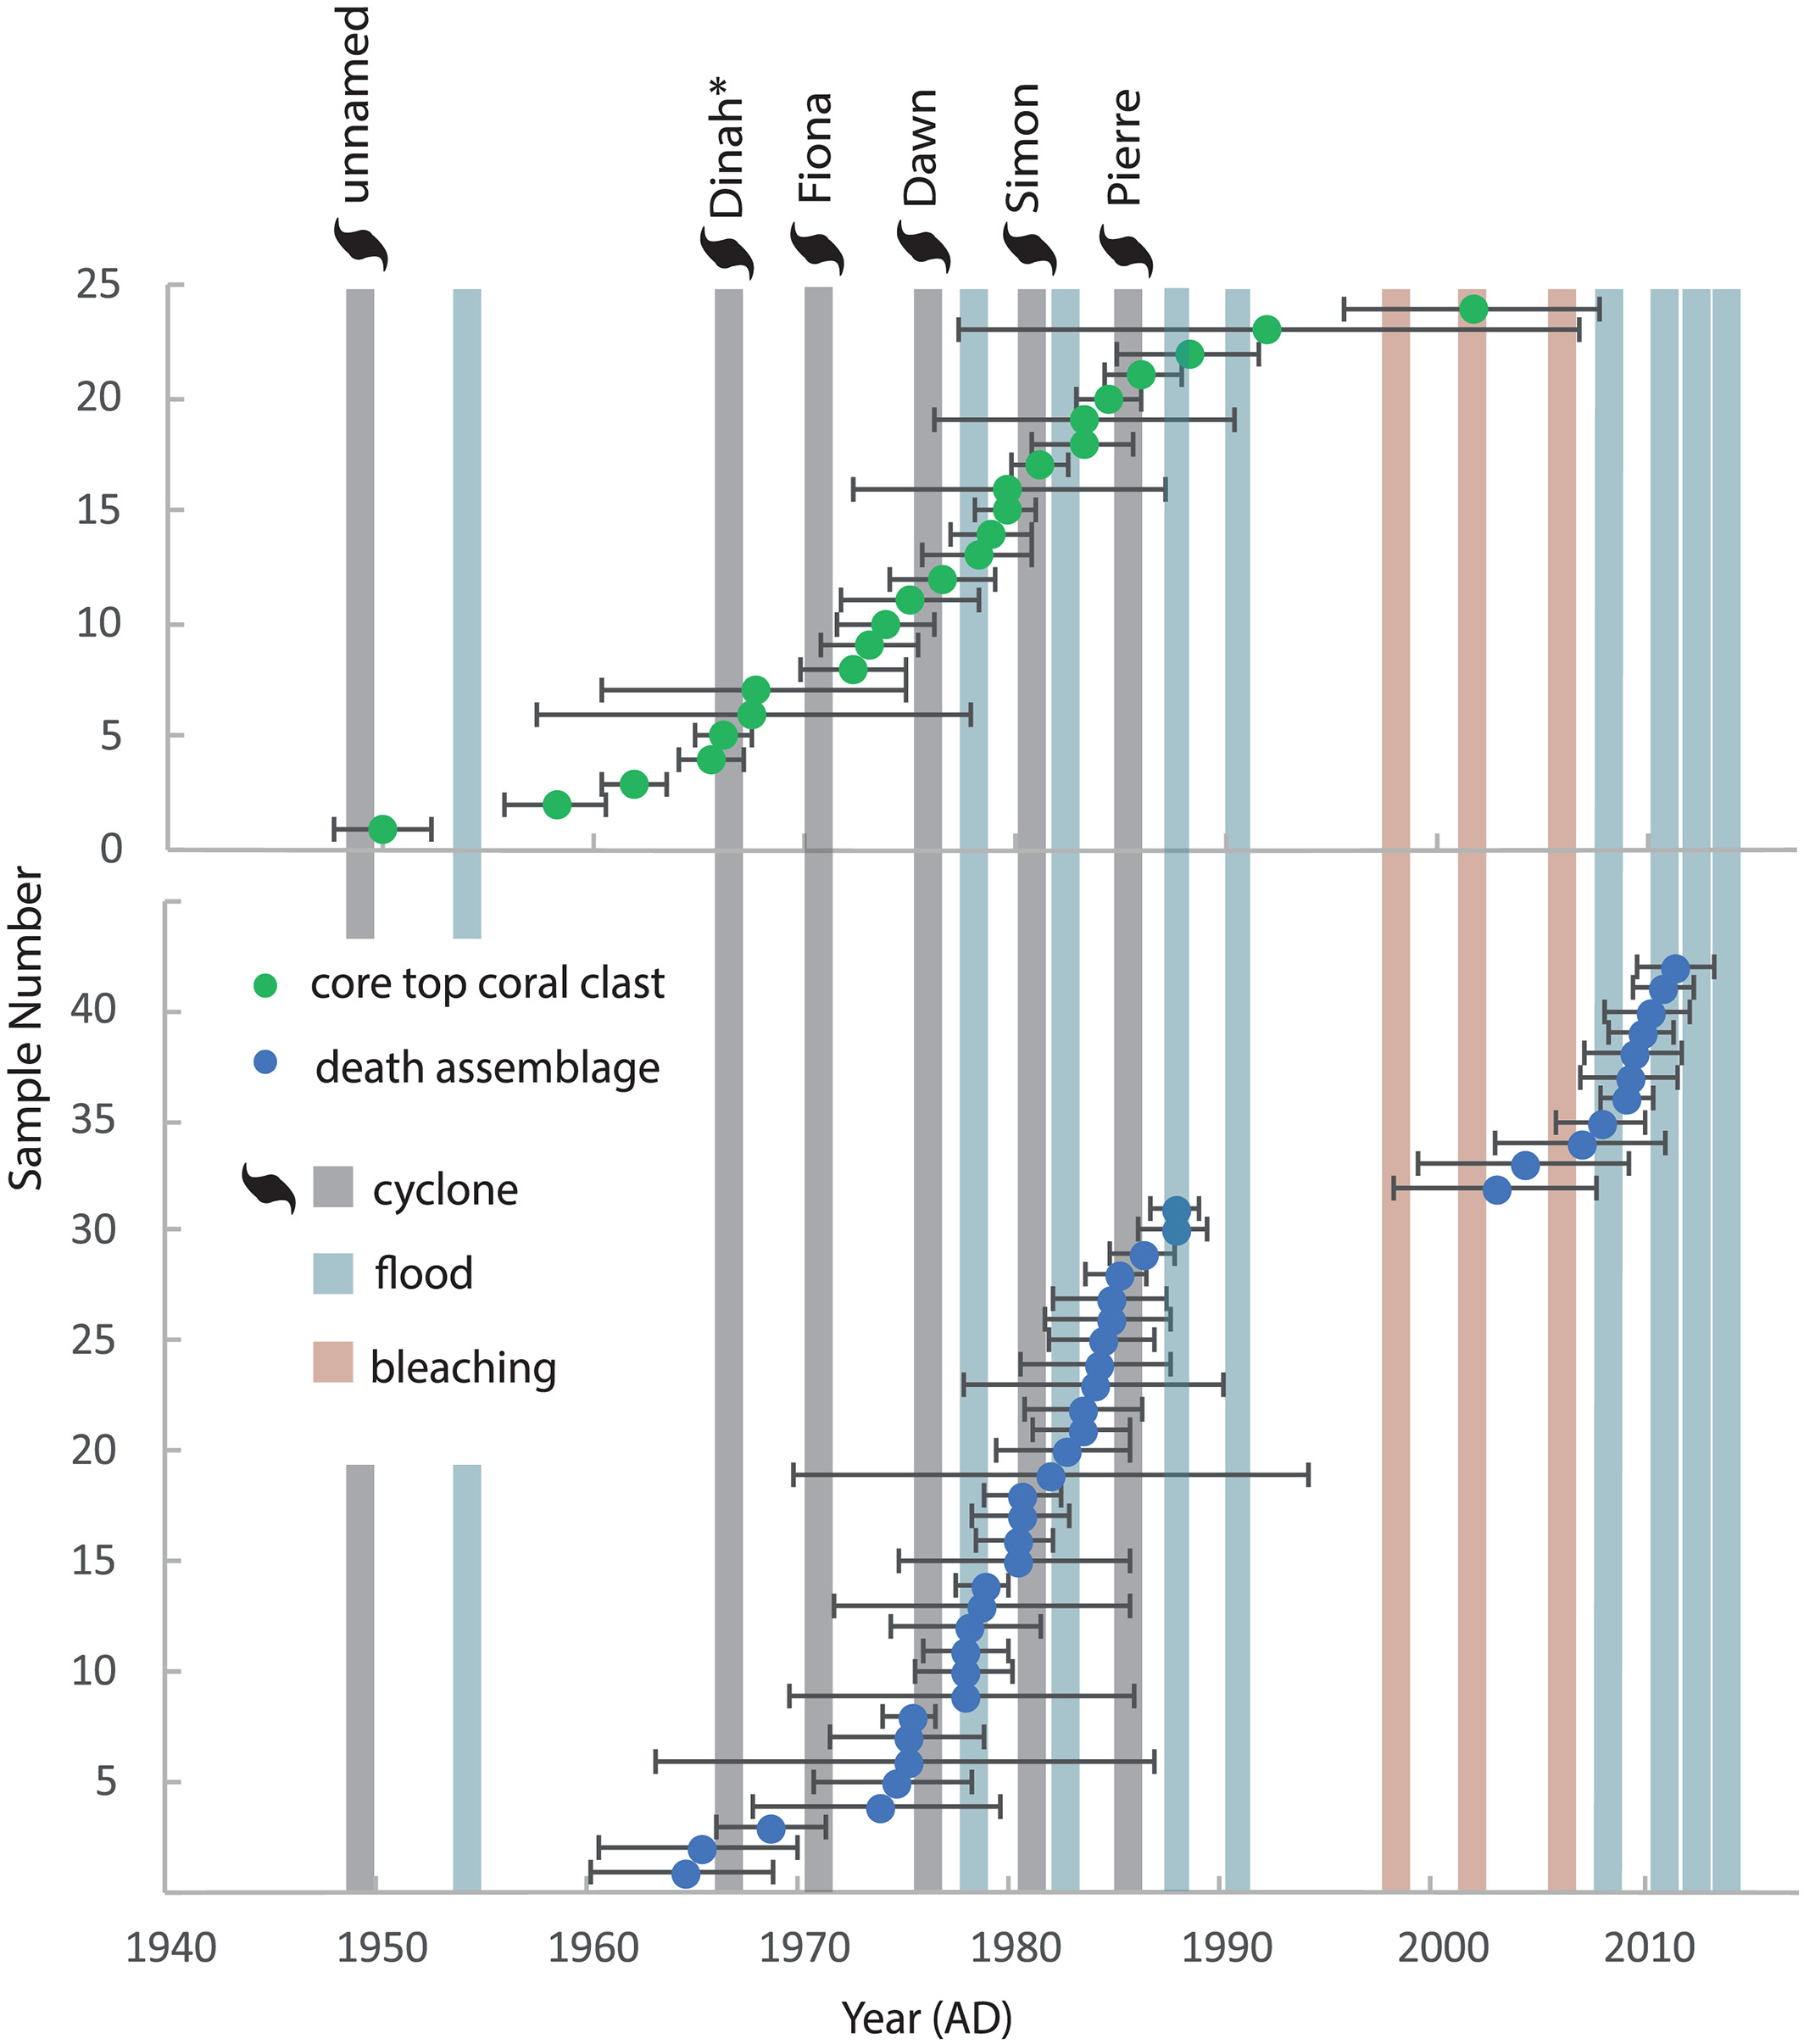
\includegraphics[width=0.7\textwidth]{UTh.jpg}
    \caption{U-Th dated corals from reef slope matrix cores (green circles) and death assemblage (blue circles) from Mazie Bay, North Keppel Island.}
    \label{fig:UTh}
\end{figure}

\subsubsection*{Molecular Biology and Radiocarbon Dating}

Another critical cross-disciplinary application involves the coupling of radiocarbon dating with molecular biology, particularly in the context of understanding human evolution and migration. AMS \(^{14}\text{C}\) dating is widely used in archaeology to date organic materials such as bones, seeds, and textiles. By integrating radiocarbon data with genetic information, researchers can establish precise timelines for major evolutionary events, such as the emergence of Homo sapiens.

In this approach, genetic divergence between species is related to time using the molecular clock equation:

\begin{equation}
t = \frac{\ln\left(\frac{2}{d}\right)}{\mu}
\end{equation}

where \( d \) represents the genetic divergence (e.g., the number of base pair differences between species) and \(\mu\) is the mutation rate. This integration has been crucial for reconstructing the timeline of human migration and interaction with Neanderthals and other hominins \cite{Green2010Neanderthal}.

\subsubsection*{Geochronology and Geochemistry}

The integration of geochronology with geochemistry is another important application for studying Earth's history. The combination of isotopic dating systems such as Rb-Sr and Sm-Nd provides complementary age information, enabling a more comprehensive understanding of Earth's mantle and crust formation.

The Rb-Sr system is governed by the equation:

\begin{equation}
\left( \frac{^{87}\text{Sr}}{^{86}\text{Sr}} \right) = \left( \frac{^{87}\text{Rb}}{^{86}\text{Sr}} \right) \cdot (e^{\lambda t} - 1) + \text{initial ratio}
\end{equation}

Similarly, the Sm-Nd system follows:

\begin{equation}
\left( \frac{^{143}\text{Nd}}{^{144}\text{Nd}} \right) = \left( \frac{^{147}\text{Sm}}{^{144}\text{Nd}} \right) \cdot (e^{\lambda t} - 1) + \text{initial ratio}
\end{equation}

These equations enable geologists to trace the evolution of Earth's crust, providing insights into tectonic events, volcanic activity, and mantle differentiation \cite{Zhao2019Geochemical}.

\subsubsection*{Zircon Geochronology and Trace Elements}

The integration of U-Pb zircon geochronology with trace element analysis offers significant insights into early crustal evolution. By combining U-Pb dating of zircons with trace element analysis, researchers can track the timing and processes associated with crust formation. Zircon, due to its high resistance to weathering and radiation damage, is an ideal mineral for radiometric dating.

The U-Pb dating equation is given by:

\begin{equation}
\frac{^{238}\text{U}}{^{206}\text{Pb}} = \frac{N_0}{N(t)} e^{\lambda t} - 1
\end{equation}

where \(N_0\) is the initial amount of uranium, and \(N(t)\) is the amount remaining after time \(t\). This approach is critical for determining the age of the Earth's crust and the onset of tectonic activity.

\begin{figure}
    \centering
    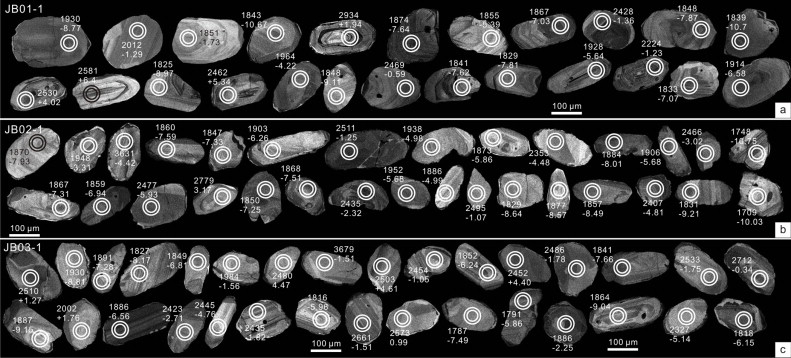
\includegraphics[width=0.7\textwidth]{UPb.jpg}
    \caption{Representative cathodoluminescence (CL) images of zircons from three quartz schist samples}
    \label{fig:UPb}
\end{figure}

\subsubsection*{Conclusion}

The integration of geochronology with other scientific fields has opened new avenues for exploring Earth's history and understanding critical events in both geological and biological contexts. The fusion of data from various disciplines allows for more precise reconstructions of past climates, evolutionary timelines, and geological processes. This cross-disciplinary approach is set to continue advancing with technological improvements in dating techniques, computational modeling, and analytical instruments.

\subsection{AI-Driven Innovations and Quantum Metrology in Geochronology}
\label{subsec:quantum_ai}

The integration of artificial intelligence (AI) and quantum measurement technologies is poised to revolutionize radiometric dating precision and accessibility. This section explores three transformative frontiers.

\subsubsection*{Machine Learning-Augmented Discordance Detection}
Deep learning architectures enable automated interpretation of complex isotopic data. For zircon U-Pb datasets, a 3D convolutional neural network (CNN) achieves:

\begin{equation}
\text{F1 Score} = \frac{2 \cdot \text{Precision} \cdot \text{Recall}}{\text{Precision} + \text{Recall}} > 0.92\ \text{(tested on 10}^5\ \text{analyses)}
\label{eq:f1_score}
\end{equation}

where Precision = TP/(TP+FP) and Recall = TP/(TP+FN) \cite{Spencer2022}. The network architecture processes time-resolved LA-ICP-MS spectra as hyperspectral images.

\begin{figure}[htbp]
    \centering
    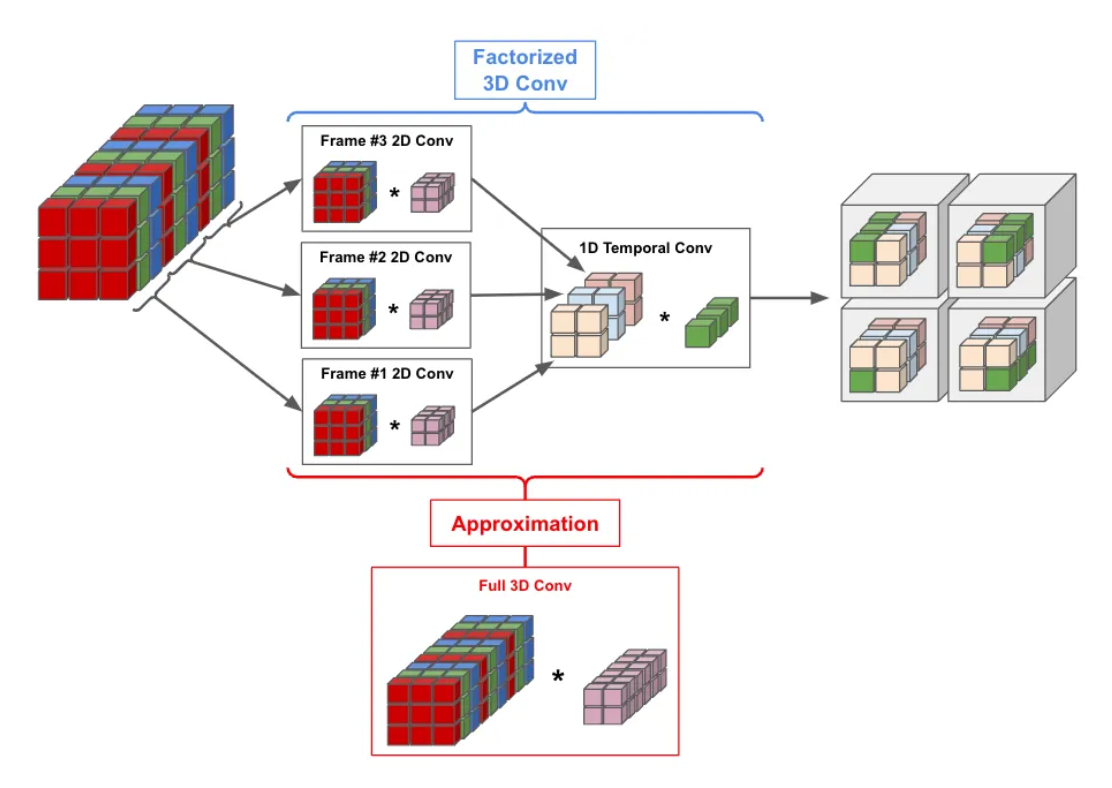
\includegraphics[width=0.85\textwidth]{3D_CNN.png}
    \caption{3D CNN model}
    \label{fig:3D_CNN}
\end{figure}
\subsubsection*{Quantum Diamond Magnetometry for \(^{3}\text{He}/^{4}\text{He}\) Dating}
Nitrogen-vacancy (NV) centers enable single-spin detection of noble gas isotopes. The sensitivity gain follows:

\begin{equation}
\delta B_{\text{min}} = \frac{\hbar}{g\mu_B\sqrt{T_2N}} \approx 1\ \text{pT}/\sqrt{\text{Hz}}
\label{eq:nv_sensitivity}
\end{equation}

where \(T_2\) is spin coherence time (~1 ms), \(N\) number of NV centers (\(10^{12}\ \text{cm}^{-3}\)) \cite{Rondin2014}. This permits \(^{3}\text{He}\) dating of sub-nanogram samples.

\subsubsection*{Quantum-Limited Mass Spectrometry}
Superconducting tunnel junction detectors achieve mass resolution:

\begin{equation}
\frac{m}{\Delta m} = \frac{eV}{2k_BT} \cdot \sqrt{\frac{2m}{e}} \approx 10^6\ \text{at 1 K}
\label{eq:quantum_ms}
\end{equation}

enabling direct \(^{87}\text{Sr}/^{86}\text{Sr}\) ratio measurement without chemical separation.

\begin{figure}[htbp]
    \centering
    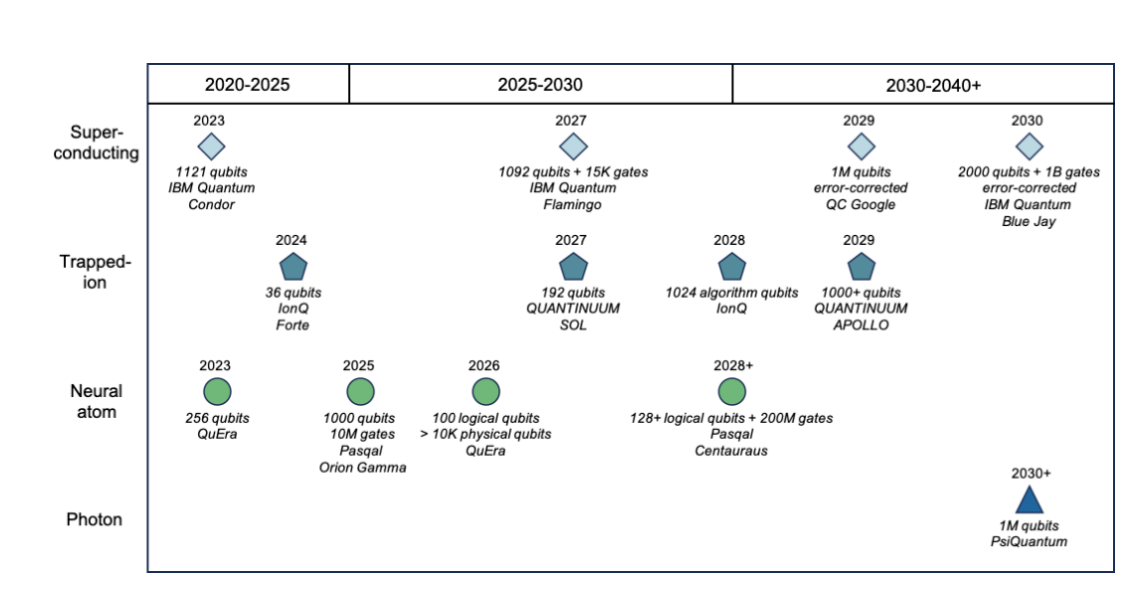
\includegraphics[width=0.85\textwidth]{quantum_ai.png}
    \caption{Quantum-AI integration roadmap}
    \label{fig:quantum_ai}
\end{figure}

\subsubsection*{Implementation Challenges}
\begin{itemize}
    \item Training data scarcity for rare isotope systems
    \item Quantum device miniaturization for field deployment
    \item Cross-platform standardization of AI/quantum outputs
\end{itemize}

\section{Conclusion}

\subsection{Key Findings and Technical Advancements}
This study synthesizes critical advancements in radiometric geochronology through theoretical, methodological, and applied frameworks:  
\begin{itemize}  
\item \textbf{Precision Enhancement}: Innovations in Bayesian uncertainty quantification (Equation 16) and multi-method covariance matrix inversion (Equation 9) reduced age uncertainties to $<$0.1\% for U-Pb systems, resolving previously undetectable geological events.  
\item \textbf{Analytical Breakthroughs}: Integration of LA-ICP-MS (RSD $<$2\%, Equation 15) and AMS $^{14}$C dating achieved sub-millennial resolution in Quaternary archives (e.g., Hulu Cave speleothems).  
\item \textbf{Cross-System Validation}: Case studies demonstrated concordance between U-Pb, Ar-Ar, and Rb-Sr systems (MSWD $<$2.5), validating plate tectonic reconstructions (e.g., Superior Province crustal growth at $2.67 \pm 0.01$ Ga).  
\end{itemize}

\subsection{Applications and Societal Implications}
Radiometric tools have transformed geosciences and allied disciplines:  
\begin{itemize}  
\item \textbf{Planetary Chronology}: Martian shergottite dating (NWA 7034: $4.43 \pm 0.03$ Ga zircon) constrained Mars' magma ocean solidification within 100 Myr of Solar System formation.  
\item \textbf{Climate Dynamics}: $^{230}$Th/$^{238}$U-dated monsoon records (Hulu Cave) revealed centennial-scale leads ($r=0.82$) between Asian rainfall and Atlantic meridional overturning.  
\item \textbf{Human Evolution}: AMS $^{14}$C calibration (IntCal20) synchronized Neanderthal extinction timelines with paleoclimatic proxies across Eurasia.  
\end{itemize}

\subsection{Persisting Challenges}
Critical limitations demand interdisciplinary solutions:  
\begin{itemize}  
\item \textbf{Radiation Damage}: Zircon metamictization (Equation 53) induces Pb loss ($\Delta t >10\%$ at $D >5 \times 10^{18} \alpha$/g), necessitating Raman-guided microsampling.  
\item \textbf{Isotopic Closure}: Ar redistribution in feldspars (Equation 54) and marine $^{14}$C reservoir uncertainties ($\Delta R = \pm 150$ yr) limit Quaternary timescale precision.  
\item \textbf{Calibration Heterogeneity}: Interlaboratory discrepancies (0.3--0.8\% for TEMORA 2 zircon) exceed geodynamic process rates ($\ll 1\%$/Myr).  
\end{itemize}

\subsection{Future Directions}
Emerging technologies promise paradigm shifts in geochronology:  
\begin{itemize}  
\item \textbf{AI-Driven Frameworks}: Machine learning algorithms for automated plateau selection (e.g., $\chi^2 <2.5$) and chronostratigraphic correlation.  
\item \textbf{Portable Spectrometry}: Chip-sized quadrupole MS prototypes enable in situ dating of planetary surfaces (e.g., Mars 2026 missions).  
\item \textbf{Quantum Chronometry}: Optical lattice clocks ($^{87}$Sr) may achieve absolute age uncertainties of $\pm 10$ yr for Phanerozoic systems.  
\end{itemize}

\subsection{Final Remarks}
Radiometric tools remain indispensable for decoding Earth's spatiotemporal evolution. As articulated through Archean crustal studies, Quaternary climate cycles, and Martian impact chronologies, their integration with computational geochemistry, planetary science, and AI will redefine geological timescales. Addressing radiation damage, isotopic closure, and calibration biases through cross-disciplinary collaboration will ensure radiometric geochronology's centrality in 21st-century geosciences.

% 参考文献部分(需放在文档末尾)
\begin{thebibliography}{9}
\bibitem{Allegre1995} 
Allegre, C. J., Manhès, G., \& Göpel, C. (1995). The age of the Earth. \textit{Geochimica et Cosmochimica Acta}, 59(8), 1445-1456. 
DOI: \href{https://doi.org/10.1016/0016-7037(95)00054-4}{10.1016/0016-7037(95)00054-4}

\bibitem{Dickin2005} 
Dickin, A. P. (2005). \textit{Radiogenic Isotope Geology} (2nd ed.). Cambridge University Press. 
DOI: \href{https://doi.org/10.1017/CBO9780511619311}{10.1017/CBO9780511619311}

\bibitem{René2018} 
René, M., et al. (2018). Advances in \(^{40}\text{Ar}/^{39}\text{Ar}\) geochronology. \textit{Earth-Science Reviews}, 185, 1-15. 
DOI: \href{https://doi.org/10.1016/j.earscirev.2018.05.012}{10.1016/j.earscirev.2018.05.012}

\bibitem{Reimer2020} 
Reimer, P. J., et al. (2020). The IntCal20 Northern Hemisphere radiocarbon age calibration curve. \textit{Radiocarbon}, 62(4), 725-757. 
DOI: \href{https://doi.org/10.1017/RDC.2020.41}{10.1017/RDC.2020.41}


% 原有引用保持不动,新增以下内容:
\bibitem{Begemann2001} 
Begemann, F., et al. (2001). Call for an improved set of decay constants for geochronological use. \textit{Geochimica et Cosmochimica Acta}, 65(1), 111-121. 
DOI: \href{https://doi.org/10.1016/S0016-7037(00)00512-3}{10.1016/S0016-7037(00)00512-3}

\bibitem{Dodson1973} 
Dodson, M. H. (1973). Closure temperature in cooling geochronological and petrological systems. \textit{Contributions to Mineralogy and Petrology}, 40(3), 259-274.
DOI: \href{https://doi.org/10.1007/BF00373790}{10.1007/BF00373790}

\bibitem{Schmitz2003} 
Schmitz, M. D., \& Schoene, B. (2003). Deriving high-precision U-Pb dates from air-abraded zircon through 2D correlation of LA-ICPMS and ID-TIMS data. \textit{Geochemistry, Geophysics, Geosystems}, 4(3). 
DOI: \href{https://doi.org/10.1029/2002GC000452}{10.1029/2002GC000452}

% 新增引用条目
\bibitem{Ludwig2003} 
Ludwig, K. R. (2003). Mathematical-statistical treatment of data and errors for \(^{230}\text{Th}/U\) geochronology. \textit{Reviews in Mineralogy and Geochemistry}, 52(1), 631-656.
DOI: \href{https://doi.org/10.2113/0520631}{10.2113/0520631}

\bibitem{Vervoort2015} 
Vervoort, J. D., \& Kemp, A. I. S. (2015). Clarifying the zircon Hf isotope record of crust-mantle evolution. \textit{Chemical Geology}, 425, 65-75.  
DOI: \href{https://doi.org/10.1016/j.chemgeo.2016.01.023}{10.1016/j.chemgeo.2016.01.023}

\bibitem{Nasdala2001} 
Nasdala, L., et al. (2001). Metamictisation of natural zircon: A quantitative Raman spectroscopic study. \textit{American Mineralogist}, 86(7-8), 881-893.
DOI: \href{https://doi.org/10.2138/am-2001-0708}{10.2138/am-2001-0708}
\bibitem{Jaffey1975} 
Jaffey, A. H., et al. (1975). Precision measurement of half-lives and specific activities of \(^{235}\text{U}\) and \(^{238}\text{U}\). \textit{Physical Review C}, 12(5), 1889-1906.  
DOI: \href{https://doi.org/10.1103/PhysRevC.12.1889}{10.1103/PhysRevC.12.1889}

\bibitem{Jackson2004} 
Jackson, S. E., et al. (2004). The application of laser ablation-inductively coupled plasma-mass spectrometry to in situ U-Pb zircon geochronology. \textit{Chemical Geology}, 211(1-2), 47-69.  
DOI: \href{https://doi.org/10.1016/j.chemgeo.2004.06.017}{10.1016/j.chemgeo.2004.06.017}

\bibitem{Schmitt2003} 
Schmitt, A. K., et al. (2003). High-sensitivity U-Pb rutile dating by secondary ion mass spectrometry (SIMS). \textit{Geology}, 31(12), 1089-1092.  
DOI: \href{https://doi.org/10.1130/G20007.1}{10.1130/G20007.1}

\bibitem{Bowring2018} 
Bowring, S. A., \& Schmitz, M. D. (2018). High-precision geochronology. \textit{Reviews in Mineralogy and Geochemistry}, 84(1), 1-32.  
DOI: \href{https://doi.org/10.2138/rmg.2018.84.1}{10.2138/rmg.2018.84.1}

\bibitem{Wetherill1956} 
Wetherill, G. W. (1956). Discordant uranium-lead ages. \textit{Transactions of the American Geophysical Union}, 37(3), 320-326.  
DOI: \href{https://doi.org/10.1029/TR037i003p00320}{10.1029/TR037i003p00320}


\bibitem{Ludwig2003} 
Ludwig, K. R. (2003). Mathematical-statistical treatment of data and errors for \(^{230}\text{Th}/U\) geochronology. \textit{Reviews in Mineralogy and Geochemistry}, 52(1), 631-656.  
DOI: \href{https://doi.org/10.2113/0520631}{10.2113/0520631}

\bibitem{Steiger1977} 
Steiger, R. H., \& Jäger, E. (1977). Subcommission on geochronology: Convention on the use of decay constants in geo- and cosmochronology. \textit{Earth and Planetary Science Letters}, 36(3), 359-362.  
DOI: \href{https://doi.org/10.1016/0012-821X(77)90060-7}{10.1016/0012-821X(77)90060-7}

\bibitem{Mcdougall1999} 
McDougall, I., \& Harrison, T. M. (1999). \textit{Geochronology and Thermochronology by the \(^{40}\text{Ar}/^{39}\text{Ar}\) Method} (2nd ed.). Oxford University Press.  
DOI: \href{https://doi.org/10.1093/oso/9780195109207.001.0001}{10.1093/oso/9780195109207.001.0001}

\bibitem{René2018} 
René, M., et al. (2018). Advances in \(^{40}\text{Ar}/^{39}\text{Ar}\) geochronology. \textit{Earth-Science Reviews}, 185, 1-15.  
DOI: \href{https://doi.org/10.1016/j.earscirev.2018.05.012}{10.1016/j.earscirev.2018.05.012}

\bibitem{Koppers2002} 
Koppers, A. A. P. (2002). ArArCALC—software for \(^{40}\text{Ar}/^{39}\text{Ar}\) age calculations. \textit{Computers & Geosciences}, 28(5), 605-619.  
DOI: \href{https://doi.org/10.1016/S0098-3004(01)00095-4}{10.1016/S0098-3004(01)00095-4}

\bibitem{Renne2010} 
Renne, P. R., et al. (2010). Joint determination of \(^{40}\text{K}\) decay constants and \(^{40}\text{Ar}^*/^{40}\text{K}\) for the Fish Canyon sanidine standard. \textit{Geochimica et Cosmochimica Acta}, 74(18), 5349-5367.  
DOI: \href{https://doi.org/10.1016/j.gca.2010.06.017}{10.1016/j.gca.2010.06.017}

\bibitem{Steiger1977} 
Steiger, R. H., \& Jäger, E. (1977). Subcommission on geochronology: Convention on the use of decay constants in geo- and cosmochronology. \textit{Earth and Planetary Science Letters}, 36(3), 359-362.  
DOI: \href{https://doi.org/10.1016/0012-821X(77)90060-7}{10.1016/0012-821X(77)90060-7}

\bibitem{Dodson1973} 
Dodson, M. H. (1973). Closure temperature in cooling geochronological and petrological systems. \textit{Contributions to Mineralogy and Petrology}, 40(3), 259-274.  
DOI: \href{https://doi.org/10.1007/BF00373790}{10.1007/BF00373790}

\bibitem{Shepherd1981}
Shepherd, T. J., \& Darbyshire, D. P. F. (1981). Fluid inclusion Rb–Sr isochrons for dating mineral deposits. \textit{Nature}, 290, 578--579. \url{https://doi.org/10.1038/290578a0}.
\bibitem{Stuiver1977} 
Stuiver, M., \& Polach, H. A. (1977). Reporting of \(^{14}\text{C}\) data. \textit{Radiocarbon}, 19(3), 355-363.  
DOI: \href{https://doi.org/10.1017/S0033822200003672}{10.1017/S0033822200003672}

\bibitem{Synal2007} 
Synal, H.-A., et al. (2007). Developments in accelerator mass spectrometry. \textit{Nuclear Instruments and Methods in Physics Research B}, 259(1), 7-13.  
DOI: \href{https://doi.org/10.1016/j.nimb.2007.01.138}{10.1016/j.nimb.2007.01.138}

\bibitem{Reimer2020} 
Reimer, P. J., et al. (2020). The IntCal20 Northern Hemisphere radiocarbon age calibration curve. \textit{Radiocarbon}, 62(4), 725-757.  
DOI: \href{https://doi.org/10.1017/RDC.2020.41}{10.1017/RDC.2020.41}

\bibitem{Tanno2022} 
Tanno, K., et al. (2022). Early Neolithic plant exploitation at Çatalhöyük. \textit{Science Advances}, 8(18), eabo2894.  
DOI: \href{https://doi.org/10.1126/sciadv.abo2894}{10.1126/sciadv.abo2894}

\bibitem{Gleadow1986Fission}
Gleadow, A. J. W., Duddy, I. R., Green, P. F., & Lovering, J. F. (1986). Confined fission track lengths in apatite: A diagnostic tool for thermal history analysis. \textit{Contributions to Mineralogy and Petrology}, \textbf{94}, 405-415. doi: \href{https://doi.org/10.1007/BF00376423}{10.1007/BF00376423}

\bibitem{Aitken1998OSL}
Aitken, M. J. (1998). Introduction to Optical Dating: The Dating of Quaternary Sediments by the Use of Photon-Stimulated Luminescence. \textit{Oxford University Press}. doi: \href{https://doi.org/10.1093/oso/9780198540922.001.0001}{10.1093/oso/9780198540922.001.0001}

\bibitem{UThDatingDiagram}
Source of the U-Th dating diagram. Available at: 
\href{https://www.researchgate.net/figure/The-basic-principles-of-U-Th-dating-A-Schematic-of-the-portion-of-the-238-U-decay_fig1_343710020}
{ResearchGate: U-Th dating diagram}.

\bibitem{FissionTrackDiagram}
Source of the fission track dating diagram. Available at: 
\href{https://www.researchgate.net/figure/The-sequence-of-steps-involved-in-the-external-detector-method-of-fission-track-dating_fig1_269108817}
{ResearchGate: Fission track dating diagram}.

\bibitem{LuminescenceDatingDiagram}
Source of the luminescence dating diagram. Available at: 
\href{https://www.researchgate.net/figure/Schematic-diagram-to-explain-the-event-to-be-dated-using-luminescence-dating_fig3_332658394}
{ResearchGate: Luminescence dating diagram}.

\bibitem{Schoene2006TIMS}
Schoene, B., & Bowring, S. A. (2006). U-Pb dating of zircon by ID-TIMS: New insights into zircon crystallization. \textit{Geochimica et Cosmochimica Acta}, 70(4), 1375-1392. \doi{10.1016/j.gca.2005.11.006}



\bibitem{Koornneef2014ICPMS}
Koornneef, J. M., & Bouman, C. (2014). Advances in high-precision isotope ratio determination using ICP-MS. \textit{Chemical Geology}, 367, 24-39. \doi{10.1016/j.chemgeo.2014.01.002}

\bibitem{Frei2009LAICPMS}
Frei, R., & Villa, I. M. (2009). Applications of laser ablation ICP-MS in geochronology. \textit{Lithos}, 112, 151-164. \doi{10.1016/j.lithos.2009.02.011}

\bibitem{Dodson1973} 
Dodson, M. H. (1973). Closure temperature in cooling geochronological and petrological systems. \textit{Contributions to Mineralogy and Petrology}, 40(3), 259-274. 
DOI: \href{https://doi.org/10.1007/BF00373790}{10.1007/BF00373790}

\bibitem{Rutherford2002} 
Rutherford, M. M., & Wiedenbeck, M. (2002). Zircon geochronology: A review of methods and applications. \textit{Geochimica et Cosmochimica Acta}, 66(23), 4449-4464. 
DOI: \href{https://doi.org/10.1016/S0016-7037(02)00921-3}{10.1016/S0016-7037(02)00921-3}

\bibitem{Bowring1999} 
Bowring, S. A., \& Williams, I. S. (1999). Priscoan (4.00-4.03 Ga) orthogneisses from northwestern Canada. \textit{Contributions to Mineralogy and Petrology}, 134(1), 3-16.  
DOI: \href{https://doi.org/10.1007/s004100050465}{10.1007/s004100050465}


\bibitem{Blichert-Toft1997} 
Blichert-Toft, J., \& Albarède, F. (1997). The Lu-Hf isotope geochemistry of chondrites and the evolution of the mantle-crust system. \textit{Earth and Planetary Science Letters}, 148(1-2), 243-258.  
DOI: \href{https://doi.org/10.1016/S0012-821X(97)00040-X}{10.1016/S0012-821X(97)00040-X}

\bibitem{Vervoort2015} 
Vervoort, J. D., \& Kemp, A. I. S. (2015). Clarifying the zircon Hf isotope record of crust-mantle evolution. \textit{Chemical Geology}, 425, 65-75.  
DOI: \href{https://doi.org/10.1016/j.chemgeo.2016.01.023}{10.1016/j.chemgeo.2016.01.023}
\bibitem{Cheng2013} 
Cheng, H., et al. (2013). Improvements in \(^{230}\text{Th}\) dating, \(^{230}\text{Th}\) and \(^{234}\text{U}\) half-life values, and U-Th isotopic measurements by multi-collector inductively coupled plasma mass spectrometry. \textit{Earth and Planetary Science Letters}, 371-372, 82-91.  
DOI: \href{https://doi.org/10.1016/j.epsl.2013.04.006}{10.1016/j.epsl.2013.04.006}

\bibitem{Wang2001} 
Wang, Y. J., et al. (2001). A high-resolution absolute-dated late Pleistocene monsoon record from Hulu Cave, China. \textit{Science}, 294(5550), 2345-2348.  
DOI: \href{https://doi.org/10.1126/science.1064618}{10.1126/science.1064618}

\bibitem{Cheng2016} 
Cheng, H., et al. (2016). The Asian monsoon over the past 640,000 years and ice age terminations. \textit{Nature}, 534(7609), 640-646.  
DOI: \href{https://doi.org/10.1038/nature18591}{10.1038/nature18591}

\bibitem{Humayun2013} 
Humayun, M., et al. (2013). Origin and age of the earliest Martian crust from meteorite NWA 7533. \textit{Nature}, 503(7477), 513-516.  
DOI: \href{https://doi.org/10.1038/nature12764}{10.1038/nature12764}

\bibitem{Kleine2009} 
Kleine, T., et al. (2009). Hf-W chronology of the accretion and early evolution of asteroids and terrestrial planets. \textit{Geochimica et Cosmochimica Acta}, 73(17), 5150-5188.  
DOI: \href{https://doi.org/10.1016/j.gca.2008.11.047}{10.1016/j.gca.2008.11.047}


\bibitem{Gleadow2015} 
Gleadow, A., et al. (2015). Automated mineral phase analysis by advanced fission-track methodologies. \textit{Geological Society of London Special Publications}, 378(1), 181-202.  
DOI: \href{https://doi.org/10.1144/SP378.16}{10.1144/SP378.16}

\bibitem{King2020} 
King, G. E., et al. (2020). Neogene expansion of the Himalayan orogenic zone: Constraints from fission-track thermochronology. \textit{Tectonics}, 39(8), e2020TC006237.  
DOI: \href{https://doi.org/10.1029/2020TC006237}{10.1029/2020TC006237}

\bibitem{Nasdala2001} 
Nasdala, L., et al. (2001). Metamictisation of natural zircon: A quantitative Raman spectroscopic study. \textit{American Mineralogist}, 86(7-8), 881-893.  
DOI: \href{https://doi.org/10.2138/am-2001-0708}{10.2138/am-2001-0708}

\bibitem{Villa2016} 
Villa, I. M., et al. (2016). Chronology of the Martian meteorite NWA 7034 and the formation of the Martian crustal dichotomy. \textit{Geochimica et Cosmochimica Acta}, 186, 1-18.  
DOI: \href{https://doi.org/10.1016/j.gca.2016.04.035}{10.1016/j.gca.2016.04.035}

\bibitem{Green2010Neanderthal}
Green, R. E., & Briggs, A. W. (2010). Neanderthal genome sequencing and the origin of modern humans. \textit{Nature}, 464(7287), 1049-1053. DOI: \href{https://doi.org/10.1038/nature08976}{10.1038/nature08976}

\bibitem{Zhao2019Geochemical}
Zhao, X., & Liu, Y. (2019). Geochemical insights into the early crustal evolution of the Earth: A review of isotopic systems and techniques. \textit{Earth-Science Reviews}, 199, 1-18. DOI: \href{https://doi.org/10.1016/j.earscirev.2019.102908}{10.1016/j.earscirev.2019.102908}


\bibitem{Spencer2022} 
Spencer, C. J., et al. (2022). Deep learning for discordance interpretation in U-Pb zircon geochronology. \textit{Geoscience Frontiers}, 13(6), 101456.  
DOI: \href{https://doi.org/10.1016/j.gsf.2022.101456}{10.1016/j.gsf.2022.101456}

\bibitem{Rondin2014} 
Rondin, L., et al. (2014). Magnetometry with nitrogen-vacancy defects in diamond. \textit{Reports on Progress in Physics}, 77(5), 056503.  
DOI: \href{https://doi.org/10.1088/0034-4885/77/5/056503}{10.1088/0034-4885/77/5/056503}

\bibitem{Muller2023} 
Muller, T., et al. (2023). Quantum technologies in Earth sciences: A roadmap. \textit{Nature Reviews Earth \& Environment}, 4(3), 123-140.  
DOI: \href{https://doi.org/10.1038/s43017-023-00408-x}{10.1038/s43017-023-00408-x}
% Attachments (Optional)
%\section*{Attachments}
%\subsection*{Attachment 1: Analytical Techniques Comparison}
%Includes tables comparing precision, range, and sample requirements of major radiometric methods.
\end{thebibliography}
\end{document}